\chapter{Editing}%
\label{cha:editing}

Editing comprises both time and track space.  The timeline consists of the time certain media appear on the track going left to right and a set of tracks from the top to the bottom.  There are 2 methods of timeline editing --- drag and drop editing, also called \textit{arrow mode}, and cut and paste editing or \textit{I-beam mode}.  Cut and Paste is the default editing mode.  An additional, but not often considered editing method is called \textit{two-screen editing} where the Viewer is used to view media and then the desired media is transferred to the timeline.

The timeline is where all editing decisions are made.  This is a stack of tracks in the center of the main window.  It can be scrolled up, down, left and right with the scrollbars on the right and bottom.  It can also be scrolled up and down with a mouse wheel, or left and right while holding down the Ctrl key and using the mouse wheel.

The active region is the range of time which is affected by editing commands on the timeline.  The active region is determined first by the presence of in/out points on the timeline.  If those do not exist the highlighted region is used.  If no highlighted region exists, the insertion point is used as the start of the active region.  Some commands treat all the space to the right of the insertion point as active while others treat the active length as 0 if no end point for the active region is defined.

Most importantly, editing decisions never affect source material meaning that it is non-destructive editing.  So not only does your original media stay completely untouched, it is much faster than if you had to copy all the media affected by an edit.  Editing only affects pointers to source material, so if you want to have a new modified media file at the end of your editing session which represents the editing decisions, you need to render it.  Saving and loading your edit decisions is explained in the Load, Save and the EDL section and rendering is explained in the section on Rendering.

In the following editing sections, references to common operations are scattered within any of the modes where they seem pertinent.  However, many of the editing operations work in different modes.

\section{The Patchbay}%
\label{sec:patchbay}

On the left of the timeline is a region known as the patchbay.  The patchbay enables features specific to each track as described next.

\begin{description}
    \item[Textbox] for naming the track.  The default names will usually be Video \#, Audio \#, or Mixer \# if using the multi-camera/mixer operations.  A \# will be designated for subsequent tracks as in 1, 2, 3 and so on.
    \item[Expander] which is a down arrow on the right side, is for viewing more options on the patchbay and for viewing the effects represented on the track.   You can just click on the expander to expand or collapse the patchbay and the track.  If it is pointing sideways, the track is collapsed.  If it is pointing down, the track is expanded.  Existing effects appear below the media for the track.
\end{description}

\noindent Below the textbox name are several toggles referred to as \textit{attributes} for different features (currently there are 5 as shown in figure~\ref{fig:patchbay}).

\begin{wrapfigure}[20]{r}{0.5\textwidth}
    \centering
    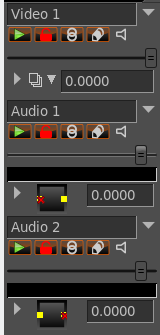
\includegraphics[width=0.6\linewidth]{images/patchbay01.png}
    \caption{Patchbay}
    \label{fig:patchbay}
\end{wrapfigure}

If the toggle button is shadowed by a color, the feature is enabled . If the toggle is the background color of most of the window, it is disabled. Click on the toggle to enable/disable the feature.

Several mouse operations speed up the configuration of several tracks at a time. Click on an attribute and drag the cursor across adjacent tracks to copy the same attribute to those tracks.  Hold down Shift while clicking a track's attribute to enable the attribute in the current track and toggle the attribute in all the other tracks. Or you can:

\begin{enumerate}
    \item hold down Shift while clicking an attribute,
    \item click until all the tracks except the selected one are disabled,
    \item then drag the cursor over the adjacent track to enable the attribute in the adjacent track.
\end{enumerate}

The \textit{attributes} are described here next.

\begin{description}
    \item[Play Track] determines whether the track is rendered or not. If it is off, the track is not rendered.  For example if you turn it off in all the video tracks, the rendered media file will have only audio tracks.  If the track is chained to any other tracks by a shared track effect, the other tracks perform all the effects in this shared track, regardless of play status of the shared track that in this particular case affects the media output but not fade and effects.
    \item[Arm Track] determines whether the track is armed or not.  Only the armed tracks are affected by editing operations. Make sure you have enough armed destination tracks when you paste or splice material or some tracks in the material will get left out.  In addition to restricting editing operations, the armed tracks in combination with the active region determine where material is inserted when loading files.  If the files are loaded with one of the insertion strategies which do not delete the existing project, the armed  tracks will be used as destination tracks.
    \item[Gang Fader] cause the fader to track the movement of whatever other fader you are adjusting by dragging either the fader or the curve on the track.  It doesn't affect the editing made with menu controls.  A fader is only ganged if the arm track is also on.  This is often used to adjust audio levels on all the tracks simultaneously.  Gang also causes Nudge parameters to synchronize across all the ganged tracks.
    \item[Draw Media] determines if picons or waveforms are drawn on the asset in the track.  You may want to disable this if you know that the media/format takes a long time to draw on the timeline.  By default it is set to on in order to see picons on the timeline.
    \item[Don’t send to output] , more commonly called \textit{mute}, causes the output to be thrown away once the track is completely rendered. This happens whether or not \textit{Play track} is on.  For example if you mute all the video tracks, the rendered media file will have a blank video track.  Mute track is represented on the timeline with a line that has the default color of blue.  Use the pulldown View $\rightarrow$ Mute to have the line displayed.  It is a keyframable attribute, but Mute track keyframing is a toggle and it has only the two values of on or off. If a track is part of a shared track effect, the output of the track with the shared track effect is overlaid on the final output even though it is routed back to another track (the shared track).  Mute track is used to keep the track with the shared track effect from overlapping the output of the source track (the shared track) where the shared track effect is not present.
    \item[Fader slider] fade values are represented on the timeline with a white curve that is keyframable.  All tracks have a fader, but the units of each fader depend on whether it is audio or video.  Audio fade values are in dB. They represent relative levels, where 0 is the unaltered original sound level, -40 is silence, -80 the minimum value set by default.  You can move fader and keyframes down to -80 but the parameter's curve won't go below -40.  For your convenience you can set a different fade range with the curve zoom.  Audio fader’s main purpose is to \textit{fade out} sound or to lower the sound level smoothly to silence, or \textit{fade in} to make sounds appear gradually instead of suddenly.  Video fade values are the percentage of opacity of the image in normal overlay mode, the percentage of the layer that is mixed into the render pipeline in the other overlay modes.
    Click and drag the fader to fade the track in and out.  If it is ganged to other tracks of the same media type, with the arm option enabled, the other faders should follow.  Hold down the Shift key and drag a fader to center it on the original source value (0 for audio, 100 for video).
    \item[mixer] in the expanded patchbay for that track designate the multi-camera mixer mode.
    \item[Overlay mode] in the expanded patchbay is used for porter-duff operations and is full explained in the section on Overlay Modes.
    \item[Nudge] is in the expanded patchbay.  The nudge value is the amount the track is shifted left or right during playback. The track is not displayed shifted on the timeline, but it is shifted when it is played back. This is useful for synchronizing audio with video, creating fake stereo, or compensating for an effect which shifts time, all without altering any edits (figure~\ref{fig:overlay}).
    
    \begin{figure}[htpb]
        \centering
        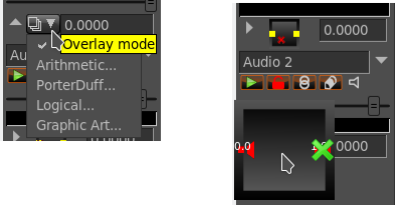
\includegraphics[width=0.7\linewidth]{images/overlay.png}
        \caption{Video Overlay, audio Pan and Nudge.}
        \label{fig:overlay}
    \end{figure}
    
    Enter the amount of time to shift to instantly shift the track. Negative numbers make the track play later. Positive numbers make the track play sooner. The nudge units are either seconds or the native units for the track (frames or samples). Select the units by right clicking on the nudge textbox and using the context sensitive menu. Nudge settings are ganged with the Gang faders toggle and the Arm track toggle. Use the mouse wheel over the nudge textbox to increment and decrement the value.
    \item[Pan] is available in the expanded patchbay for audio tracks via a panning box. Position the pointer in the panning box and click/drag to reposition the audio output among the speaker arrangement. The loudness of each speaker is printed on the relative icon during the dragging operation. The panning box uses a special algorithm to try to allow audio to be focused through one speaker or branched between the nearest speakers when more than 2 speakers are used.  
\end{description}

Press the Tab key while the cursor is anywhere over a track to toggle the track arming status. Press Shift-Tab while the cursor is over a track to toggle the arming status of every other track.

\paragraph{Automatic audio mappings}
Several convenience functions are provided for automatically setting the panning to several common standards. They are listed in the Audio menu. These functions only affect armed audio tracks. They are:

    \begin{description}
        \item[Audio$\rightarrow$Map 1:1] This maps every track to its own channel and wraps around when all the channels are allocated. It is most useful for making 2 tracks with 2 channels map to stereo and for making 6 tracks with 6 channels map to a 6 channel sound card.
        \item[Audio$\rightarrow$Map 5.1:2] This maps 6 tracks to 2 channels. The project should have 2 channels when using this function. Go to Settings $\rightarrow$ Format to set the output channels to 2. This is most useful for down-mixing 5.1 audio to stereo.
    \end{description}

\paragraph{Standard audio mappings} Although Cinelerra lets you map any audio track to any speaker, there are standard mappings you should use to ensure the media can be played back elsewhere. Also, most audio encoders require the audio tracks to be mapped to standard speaker numbers or they will not work.

In the channel position widget, the channels are numbered to correspond to the output tracks they are rendered to. For stereo, the source of channel 1 needs to be the left track and the source of channel 2 needs to be the right track.  For 5.1 surround sound, the sources of the 6 channels need to be in the order of center, front left, front right, back left, back right, low frequency effects. If the right tracks are not mapped to the right speakers, most audio encoders will not encode the right information if they encode anything at all. The low frequency effects track specifically can not store high frequencies in
most cases.

\section{Manipulating Tracks}%
\label{sec:manipulating_tracks}

Tracks in Cinelerra either contain audio or video.  There is no special designation for tracks other than the type of media they contain.  When you create a new project, it contains three default tracks: one video track and two audio tracks.  You can still add and delete tracks from the menus.  The Tracks menu contains a number of options for dealing with multiple tracks simultaneously.  Each track itself has a popup menu which affects one track. 

Operations in the \textbf{Tracks pulldown} affect only tracks which are armed.

\begin{description}
    \item[Move tracks up | Move tracks down] shift all the armed tracks up or down the stack.
    \item[Delete tracks] deletes the armed tracks.
    \item[Delete last track] deletes the last track, whether it is armed or not.
    \item[Concatenate tracks] operation copies all the assets of every disarmed but playable track and concatenates it by pasting those assets at the end of the first set of armed tracks. They are pasted one after the other, keeping the same order they have on the stack. If there are two armed tracks followed by two disarmed tracks, the concatenate operation copies the assets of the two disarmed tracks and pastes them after the assets of the two armed tracks. If there are three disarmed tracks instead, the assets of two tracks are pasted after the assets of the armed tracks and the assets of the third track are pasted at the end of the first armed track. The destination track wraps around until all the disarmed tracks are concatenated. Disarmed tracks that are not playable are not concatenated.
    \item[Append to project] allows for creating new tracks after any existing tracks.
    \item[Add subttl] will add a track for subtitles at the top of the other tracks.
\end{description}

The \textbf{Audio} and \textbf{Video pulldowns} each contain an option to add a track of their specific type. In the case of audio, the new track is put on the bottom of the timeline and the output channel of the audio track is incremented by one. In the case of video, the new track is put on the top of the timeline. This way, video has a natural compositing order. New video tracks are overlaid on top of old tracks.

\section{Two Screen Editing}%
\label{sec:two_screen_editing}

This is a fast way to construct a program out of movie files. The idea consists of viewing a movie file in one window and viewing the program in another window. Subsections of the movie file are defined in the viewer window and transferred to the end of the program in the program window.  Two screen editing can be done simply by using keyboard shortcuts.  To get familiar with which keys to use, move the mouse pointer over the transport panel and a tooltip appears, showing what key is bound to that button.

To begin a two screen editing session, load your media resources by using the main menu \textbf{File pulldown} and choose \textit{Load files}; make sure the insertion mode is set to \textit{Create new resources only}.  This insertion strategy is to ensure that the timeline stays unchanged while new resources are brought in. Go to the Resources window and select the Media folder. The newly loaded resources will appear. Double click on a resource or drag it from the media side of the window over to the Viewer window.

Check to make sure there are enough armed tracks on the timeline to put the subsections of source material that you want.  Usually this would be one video track and two audio tracks, but if there are not enough, just create new tracks or arm more tracks.

Now to start your 2 screen editing, in the viewer window, define a clip from the media file:

\begin{enumerate}
    \item Set the starting point with the In pointer button.  You will see a left hand bracket on the timebar.
    \item Move your cursor to the ending point of the clip you want to use.
    \item Set the ending point with the Out pointer right hand bracket.
\end{enumerate}

\noindent These In/Out points define a clip.  You can now use this in a couple of different ways.

\paragraph{Splice} The splice icon, or shortcut letter “v”, inserts the selected area in the timeline after the insertion point.  After the splice has taken effect, the insertion point moves to the end of the edit ready to be used as the next splice location. This way you can continuously build up the program by splicing.
If an In point or an Out point exists on the timeline the clip is inserted after the In point or after the Out point. If both In and Out points are set on the timeline, the clip is inserted after the In point. If there are edits after your chosen splice location on the timeline, they will be moved to the right.

\paragraph{Overwrite} The overwrite icon, or shortcut letter “b”, overwrites the region of the timeline after the insertion point with the clip. If an In point or an Out point exists on the timeline the clip is overwritten after the In point or after the Out point. If both In and Out points are set on the timeline, the clip is inserted after the In point. If a region is highlighted or both In and Out points exist they limit the region of the overwriting and the clip may therefore be shortened. Here is a detailed explanation to take advantage of this method.

To overwrite exactly on a precise region of the timeline:

\begin{enumerate} [noitemsep]
    \item Arm only tracks to change.
    \item Define the destination region on the timeline with [ and ], the In and Out points.
    \item Define the clip you want to use in the viewer with [ and ], the In and Out points.
    \item Overwrite from Viewer to the timeline.
\end{enumerate}

If the destination region is shorter than the clip defined in the viewer, the portion of the clip longer than the destination region won't be inserted and on the timeline the following edits won't move.
If the destination region is longer than the clip defined in the viewer, the destination region will shrink and on the timeline the following edits will move to the left.

\paragraph{Clip} The clip icon, or shortcut letter “i”, generates a new clip for the resource window containing the affected region but does not change the timeline.  Every clip has an optional/default title and description.

\paragraph{Copy} The copy icon, or shortcut letter “c”, copies the selection into the copy buffer.

\section{Cut and Paste Editing}%
\label{sec:cut_paste_editing}

This is the more traditional method of editing and therefore is the default.  To enable the cut and paste editing mode on the timeline, select the I-beam toggle on the control bar at the top of the main program window. You can copy edits in the same track, copy from different tracks in the same instance, start a second instance of Cinelerra and copy from one instance to the other or load a media file into the Viewer and copy from there.

To start editing, load some files onto the timeline.  Select a region of the timeline by click dragging on it and select the cut button to cut it. Move the insertion point to another point in the timeline and select the paste button.  Assuming no In/Out points are defined on the timeline this performs a cut and paste operation.

Most editing operations are listed in the Edit pulldown. Some of them have a button on the program control toolbar as well as a keyboard shortcut.  The keyboard shortcut is in parenthesis here.

\begin{description}
    \item [Split | Cut] (x) Delete the selected area and put it in the cut buffer for future pasting.
    \item[Copy] (c) Copy the selected area and put it in the cut buffer for future pasting.
    \item[Paste] (v)  Paste the material that is in the cut buffer.
    \item[Clear] (Del)  Clear the selected area. If the insertion point is over an edit boundary and the edits on
    each side of the edit boundary are the same resource, the edits are combined into one edit comprised
    by the resource. The start of this one edit is the start of the first edit and the end of this one edit is the
    end of the second edit. This either results in the edit expanding or shrinking.
    \item[Paste silence] (Shift+Space)  Paste blank audio/video for the length of the selected area. Following
    edits will be pushed to the right.
    \item[Mute Region] (m)  Overwrite blank audio/video on the selected area. Following edits don't move.
    \item[Trim Selection] Delete everything but the selected region.
    \item[Select All] (a) Select the whole timeline.
\end{description}

In Cut and Paste editing mode you can \textit{edit labels} as well. By enabling Edit labels in the \textbf{Settings pulldown}, or by disabling the Lock labels from moving button on the Program Control Tool Bar, labels will be cut, copied or pasted along with the selected regions of the armed tracks.

Using labels and In/Out points are useful in editing audio.  You can set In/Out points for the source region of the source waveform and set labels for the destination region of the destination waveform. Perform a cut, clear the In/Out points, select the region between the labels, and perform a paste.

\paragraph{In / Out Points} The In and Out bracket placement is explained here to illustrate their usage.  Because of the shape of the markers"[" and "]" you may assume that they are inclusive --- that everything placed in between would be included in the clip, such as in the case of being transferred to the timeline from the Viewer.  In reality, one of the two markers will not include the frame that was visible at the time the marker was affixed. Depending on whether the \textit{Always show next frame} option is used or not, it is the In or Out marker that will not be inclusive. 

To obtain a clip on the timeline exactly as you saw in the Viewer, you must necessarily move the In mark back from the beginning before the first desired frame or move the Out mark forward after the last desired frame, depending on the \textit{Always show next frame} setting. 

Some of the confusion can be attributed to the fact that the Viewer shows frames, while the markers determine spaces, i.e. times, that are not visible between frames. You have to think of each frame as being delimited by two spaces - one preceding and one following.  The In mark is always placed before the displayed frame and the Out mark is always placed after the displayed frame, while taking into account in its calculations whether the \textit{Always show next frame }option is used or not. If you just remember that the reference of the markers is in the middle of the icon, you will avoid confusion.

\paragraph{Overwrite} To perform overwriting within the timeline paste on a selected region (highlighted or
between In/Out points). The selected region will be overwritten. If the clip pasted from the clipboard
is shorter than the selected region, the selected region will be shrunk. Following edits will move. If 
the clip pasted from the clipboard is longer than the selected region, the selected region will be
overwritten with the first part of the clip and the remaining part of the clip will be written after the
overwriting. Following edits will move.

\paragraph{Tracks $\rightarrow$ Concatenate tracks} This operation copies all the assets of every disarmed but playable
track and concatenates it by pasting those assets at the end of the first set of armed tracks. They are
pasted one after the other, keeping the same order they have on the stack.

\paragraph{Split --- blade cut and hard edges:} You can cut the tracks into 2 pieces on the timeline by putting the hairline cursor on the place you want to do a cut and then using the character “x” or the scissors tool (figure~\ref{fig:cut}). 

\begin{wrapfigure}{r}{0.4\textwidth}
    \centering
    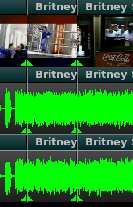
\includegraphics[width=0.7\linewidth]{images/cut.png}
    \caption{Blade cut}
    \label{fig:cut}
\end{wrapfigure}

 A \textit{cut} uses a non-empty selection region, where the \textit{blade cut} or \textit{split} has no duration in the selection, just a hairline.  As usual the use of cut when a selection is set, deletes/cuts the highlighted area.  In the case where an In point or an Out point exists on the timeline, the clip is split at the location of the In/Out point since it has priority over the cursor location.  A blade cut simply splits the edit into two edits.  In order to have the video and audio aligned, it works best to have Settings $\rightarrow$ Align cursor on frames.  When a blade cut occurs, the edges are created as \textit{hard edges}.  These are edges that cannot be deleted by track optimizations.

When you do a blade cut/split, all armed tracks will be included in the cut and green-colored triangles will show on the bottom of the track on both the left and the right side of the cut.  This is a \textit{hard edge} marker toggle, as opposed to the soft edge designation for an ordinary edit.  The \textit{hard edge} marker can be toggled off/on if so desired.  In order to not interfere with the usual drag handles, only a few pixels are used for the toggle so you have to be sure you have the cursor right over the hard edge triangle  --- when in position, it will be obvious because you can see an arrow pointing to the corner.  Use Shift-left mouse button 1 to toggle off/on the hard edge marker on all tracks simultaneously.

\section{Drag and Drop Editing}%
\label{sec:drag_drop_editing}

To enable the drag and drop editing mode on the timeline, select the arrow toggle on the control bar at the top of the main program window.  Drag and drop editing is a quick and simple way of working in Cinelerra, using mostly only the mouse. The basic idea is to create a bunch of clips, then drag them in order into the timeline, thus building prototype media that you can watch in the compositor. If after watching it, you wish to re-arrange your clips, set effects, add transitions or insert/delete material, just drag and drop them on the timeline. 

To simply get started, perform the following operations which are useful for working in a drag and drop editing session.  First load your media by using the main menu File pulldown and choose \textit{Load files}; make sure the insertion mode is set to \textit{Create new resources only}.  This loads the files into the Resources window.

\begin{enumerate}
    \item Create some video and audio tracks on the timeline using the Video and Audio pulldowns.
    \item Open the Media folder in the Resources window.  Make sure the necessary tracks are armed and drag
    a media file from the Resources window to the timeline. If the media has video, drag it onto a video 
    track or if just audio, drag it onto an audio track. For a still image, drag it onto a video track.
\end{enumerate}

\noindent You can also drag multiple files from the Resources window. When dropped in the timeline they are concatenated. If you have \textit{Display Icons} selected in the Resources window, drawing a box around the files selects contiguous files. If you have \textit{Display Text} selected, Ctrl-clicking on media files selects additional files one at a time; Shift-clicking on media files extends the number of highlighted selections.  In addition to dragging media files, if you create clips and open the clip folder you can drag
clips onto the timeline.

Cinelerra fills out the audio and video tracks below the dragging cursor with data from the file. This affects what tracks you should create initially and which track to drag the media onto. To drag and drop a file on the Program window, you need to create on the timeline the same set of tracks as your media file.

When you drag your chosen media from the media folder to the timeline, your mouse pointer will drag a thumbnail and, once over the timeline, the outline of a white rectangle, as big as the edit you are going to have appears.  Drag the media to the desired position of an empty track of the timeline and drop it.  If there are other edits on that track, when you move the white outline over an edit, you will see a bow tie symbol $\rhd\lhd$ appearing at edit boundaries. If you drop the media there, the new edit will start from the edit boundary indicated by the center of the bow tie $\rhd\lhd$.

Since the mouse pointer is in the middle of the white outline, when this rectangle is bigger than the visible part of the timeline, it is quite cumbersome to precisely insert it for long media. Lengthening the duration visible in the timeline by changing the sample zoom in the zoom panel will reduce the size of the white rectangle, making a precise insertion possible.

\noindent When you drag and drop edits within the timeline:

\begin{itemize}
    \item If you drop an edit when bow ties $\rhd\lhd$ are shown, that edit will be cut and pasted starting at the edit
    boundary indicated by the center of the bow tie $\rhd\lhd$.  Following edits on the same track will move.
    \item If you drop an edit when there are no bow ties $\rhd\lhd$ shown, the original edit will be muted and pasted
    where you dropped it. No edits will move. A silence will appear in place of the original edit.
    \item If you have more armed tracks on the timeline than in the asset you are dragging, only the following
    edits of the tracks affected by the drag and drop operation will move to the right. This will cause loss
    of synchronization. To restore it, disarm the tracks affected by the drag and drop operation, highlight
    the just dropped edit and paste silence over it using the Edit pulldown, \textit{Paste Silence}.
\end{itemize}

\noindent Labels sometimes work differently in Drag and Drop editing mode in that you can't drag and drop them. They might be locked to the timebar, even with the Edit labels option enabled.  Although with the Edit labels option enabled, if a selected area of a resource is spliced from the Viewer to the timeline in a position before labels, these labels will be pushed to the right for the length of the selected area.

In/Out points can be used to perform Cut and Paste operations in Drag and Drop mode as well as in Cut and Paste mode.  Use the Edit pulldown to view the list and their keyboard shortcuts.

\subsection{Copy/Paste Behavior}%
\label{sub:copy_paste_behavior}

There are many options for moving, copying, pasting, inserting, and deleting selected \textit{edits}, more commonly referred to by the user as \textit{clips}, when in the Drag and Drop (arrow) editing mode.  This makes it easier to avoid constantly having to disarm/arm tracks.  To create a selection move the cursor over the clip and just click the left mouse button; remove a selection by left mouse button click again.  This will mark your selection with a colored border which contains some red.  The easiest way to initially use the various modes is to click on the middle mouse button when your cursor is over a track and a popup displays the modes and shortcuts.  However, for those users who prefer the addition of the Ctrl key to add multiple selections as is commonly done for listbox operations, there is a preference in Settings $\rightarrow$ Preferences $\rightarrow$ Appearance tab, called \textit{Clears before toggle} that changes the behavior.

When an edit is marked as selected, it can be cut/copied into the paste clip buffer.  The constructed clip buffer will begin with the leftmost edit and end with the rightmost edit.  The edits may contain media, or be silence, or skipped if they are not selected.  The clip tracks are copied from the first track with an active edit selection to the last track with an active edit selection.  A clip track can be completely empty if no selection was made on the track.  The word \textit{packed} means that the silent edits and empty tracks are not included in the copy to the clip buffer, and all of the elements are packed together, no gaps.  Packing a clip buffer makes it easier to move \textit{blobs} of data around.  Once the edits have moved and have a relative relationship applied, an unpacked clip buffer allows the media to be copied with the relative positions of the edits preserved.

The \textit{edits} popup is activated on a track and a red and yellow colored reticle appears to temporarily mark the location when you click on the middle mouse button.  An expanded explanation is provided below.

\begin{center}
    \begin{tabular}{l p{12cm}}
        \toprule
        \textbf{Key} & \textbf{Operations} \\ \hline
        Drag & Hold down the Ctrl key while dragging to move a single edit elsewhere. \\
        Left mouse button & Selects and highlights the edit under the cursor with a red selection box. Left mouse button also will toggle that clip selection off if it is on. \\
        \bottomrule
    \end{tabular}
\end{center}

\begin{center}
    \begin{longtable}{l l p{11cm}}
        \toprule
        \textbf{Popup Label} & \textbf{Key} & \textbf{Operation} \\ \midrule
        \endhead
        Clear Select & Ctrl-Shift-A & Deselect all selected edits ---ones that have the red lines around them. \\
        Copy & Ctrl-c & Copy the selected edits into the copy buffer. \\
        Cut & Ctrl-x & Delete the selected edits after copying them into the buffer.  The edits \\
        Mute & Ctrl-m & Delete the selected edits after copying them into the buffer.  The space
        previously occupied by the edits will be replaced with silence.\\
        Copy Pack & Ctrl-Shift-C & Copy the selected edits into the buffer and remove any silent sections.\\
        Cut Pack &	Ctrl-z	&	Delete the selected edits after copying them into the buffer.  The edits after the election will move left to occupy the vacated space.  The edits in the copy buffer will be packed together within each track. \\
        Mute Pack &	Ctrl-Shift-M &	Delete the selected edits after copying them into the buffer.  The deleted
        edits will be replaced with silence.  The edits in the copy buffer will be packed together within each track. \\
        Paste 	&	Ctrl-v	&	Paste contents of the copy buffer at the insertion point marked by the red \& yellow reticle of the popup menu or the position of the hairline cursor.
        This is a splice operation which creates space for the edits. \\
        Overwrite &	Ctrl-b	&	Paste contents of the copy buffer at the insertion point marked by the red \& yellow reticle of the popup menu or the position of the hairline cursor.
        This destroys the current edits in that space. \\
        Overwrite &	Ctrl-Shift-P &	Pastes plugins that are in the Copy buffer to current location but no clip.
        Plugins. \\ \bottomrule
    \end{longtable}
\end{center}
The copy/paste behavior respects the armed/disarmed tracks state.  A paste of audio on a video track will fail and vice versa.  In addition if you attempt to paste edits consisting of more tracks than what is available at that location it will not allowed.

Attaching transitions to multiple selected edits via the Video or Audio pulldowns is also available.  The new transitions are attached at the start of the edits, and will replace any existing attached transitions.

\subsection{Copy/Paste Behavior}%
\label{sub:copy_paste_behavior}

Cinelerra recognizes as a group, the edits of different armed tracks that have aligned beginnings, regardless of whether they have the same source or aligned ends.  You can drag these edits around on the timeline to construct your movie by rearranging scenes. If more than one track is armed, Cinelerra will drag any edits which start on the same positions the edit the mouse pointer is currently over. \\
Another method of Grouping of edits is performed as follows:
\begin{enumerate}
    \item Select each of the clips you would like to be part of a group.
    \item Use the desired Copy mode as described above to get into the buffer.
    \item Go to the Resources window Clip folder and right click on an empty spot.
    \item Choose the Paste Clip option.  Now you have a named clip of the current selection.
\end{enumerate}
A more traditional Grouping of edits which make a Permanent Group works as described next.  A temporary group is just a set of selected clips and works the same as a single selection.
\begin{enumerate}
    \item Create a group:
    \begin{itemize}[noitemsep]
        \item Select multiple clips/edits with left mouse button over the clip;
        \item Hold down shift and left mouse click over any of the selected clips to create a group;
        \item A Group Id and color are assigned to this group making it easy to distinguish.
    \end{itemize}
    \item Move a group:
    \begin{itemize}[noitemsep]
        \item Move your cursor over any of the clips within the group;  click to select the clip group.
        \item Click and Hold down the left mouse button to drag.
    \end{itemize}
    \item Dissolve a permanent group:\\
    To ungroup select any of the group edits/clips and shift left mouse click to ungroup (same as creating).
    The edits will be ungrouped, and the current selection will be replaced with the ungrouped clips.
\end{enumerate}
The color of the created groups are not muted and are assigned by Group Id going sequentially through the number of 1 to 64.  Therefore if you dissolve a group and make it again, it will have a different Group Id and a different color.

\subsection{Dragging Groups}%
\label{sub:dragging_groups}

Dragging while in \textit{Drop and Drag editing mode} (arrow mode) is really easy.  Just select the clip or clips you want to drag using the left mouse button, then put your cursor over one of them and drag while holding down the left mouse button.  Keyframes, autos, labels, and plugins will also be dragged.   Dragging honors armed/disarmed tracks.  When you drag there will be 3 possible colors as defined:
\begin{itemize}
    \item Red color means can not drop here because it will not fit in the space.
    \item Green color means OK to drop in that position.
    \item Yellow color means you can drop here and when you do it will be exactly next to that existing edit.
\end{itemize}
The original (older) method of dragging while in Arrow mode, lets you just left mouse click on a single clip or aligned clips and just drag.  This older method of dragging does not move any of its effects with it at this time.  There will only be a white outline while dragging and it will let you drop only if it fits.  You can also perform some dragging and grouping while in the \textit{Cut and Paste editing mode} (ibeam mode) by taking advantage of the Ctrl button in conjunction with the left mouse button.
\begin{itemize}
    \item Double click selects a column so you can move, for example, the audio and video together by holding
    down the Ctrl key and dragging.
    \item A single clip can be dragged without any of its aligned clips, by holding down and Ctrl key and drag.
\end{itemize}
This last section on Dragging, outlines the difference between \textit{column selection} and \textit{marking selection}.  Column selection is available to make it easy to still be able to do some dragging in I-beam mode whereas Marking selection makes it easy to drag clips together that are not columnated.

\section{Inter-View Mode / Identifying Source Targets Editing}%
\label{sec:inter-view_identifying_source_target_editing}

Inter-View mode provides a mapping of a particular media file to its timeline usages. It is somewhat similar to Two Screen Editing in that you make use of the Viewer. It makes it possible to precisely trace and indicate in the media the origin of a particular segment of the timeline and visually indicate the use and distribution that the timeline makes of a particular media.   A good example usage would be in the case of a 30 minute interview where you use a few short pieces to make a shorter 10 minute section, find out that you have made the timeline 12 minutes instead and need to cut out another 2 minutes. \\
This feature provides the following capabilities:
\begin{itemize}
    \item You can see on the timeline all of the places where a particular piece of media was used.
    \item You can see which parts of that particular media are already used so you do not reuse that same 
    piece again.
\end{itemize}
Figure~\ref{fig:inter-view01} shows an example of the Inter-View mode mapping preview mini-window..
\begin{figure}[htpb]
    \centering
    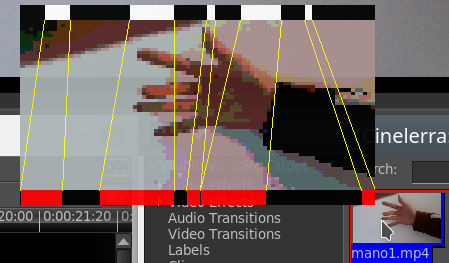
\includegraphics[width=0.8\linewidth]{images/inter-view01.png}
    \caption{Inter-View mode: white bar$\rightarrow$source; red bar$\rightarrow$timeline}
    \label{fig:inter-view01}
\end{figure}

\noindent Explanation of how to use Inter-View mode will be described here next.

\begin{itemize}
    \item Do your editing as usual on the timeline until you are ready to see what is used or unused.
    \item Make sure you are in Preview mode in the Resources window; you enable this mode using the menu
    \textit{Full play} to the left of the word Search \quad
    
\includegraphics[height=\baselineskip]{images/fullplay.png}.   \item Middle mouse click on a thumbnail in the Resources window and a popup occurs of that media with a
    white colored bar at the top and a red colored bar at the bottom with black sections.
\end{itemize}
The red/white bars represent the presence and the black sections represent the absence of where that media is used on the timeline.  To get to a bigger representation, use the “f” key for a full screen.  Now
you can operate the following buttons to display what you need to see and to move around.  It is important to note that \textit{locked tracks} will not be represented.  This makes it easy to ignore the audio track segments if you want so there is less confusion in the display.
\begin{itemize}
    \item Clicking on the top white or black spaces in the top time bar loads the Viewer with the source media,
    and sets the In/Out "[" and "]" pointers to be the selection of that edit.
    \item Click on a location in the bottom red or black bar, and the main cursor and composer will re-position
    to the corresponding location on the session timeline.
    \item Dragging on the red/black bar will correspondingly update the position in the timeline and composer.
    \item Ctrl-click on the bottom bar and the timeline and composer are re-positioned to the beginning of that
    edit.
    \item Shift-click on the bottom bar and a \textit{selection} is made of that section in the timeline and the composer
    is updated with that start position.
\end{itemize}
Figure~\ref{fig:inter-view02} displays Inter-View window and its relation to the timeline, viewer, and compositor.
\begin{figure}[htpb]
    \centering
    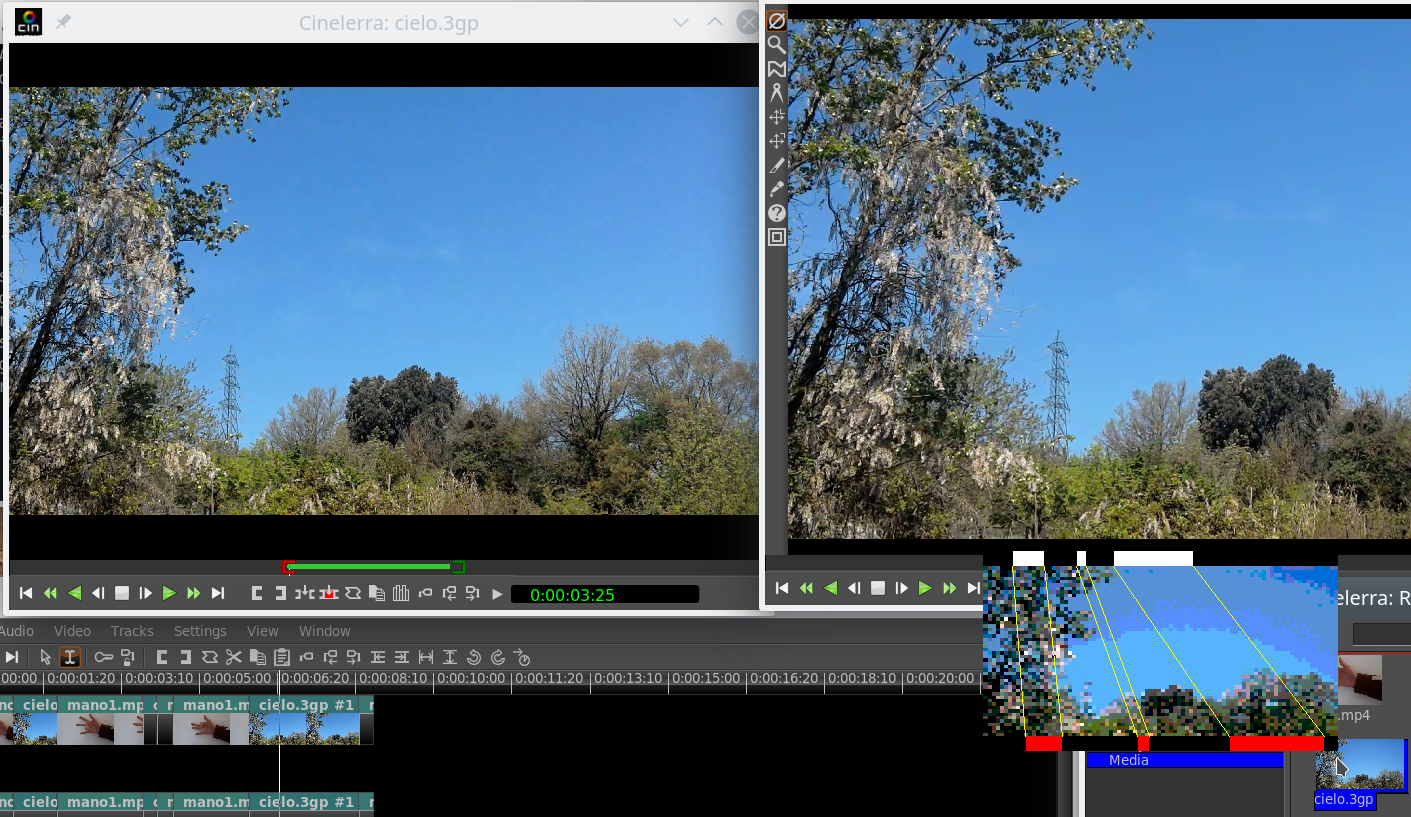
\includegraphics[width=0.9\linewidth]{images/inter-view02.png}
    \caption{Inter-View mode and the timeline}
    \label{fig:inter-view02}
\end{figure}
The Inter-View mode works for Media, Proxy, and User Bins.  When the preview window has only black bars on the top and bottom, it means that this particular media is not loaded in the timeline.  So when you are in Proxy, meaning that the Proxy files are loaded on the timeline, there will be only black bars for the corresponding Media file UNLESS there is an audio track associated with the video.  Because audio tracks are not proxied, they will show for Media but not for Proxy.

\section{Some Specific Editing Tools}%
\label{sec:specific_editing_tools}

\noindent This section covers some more detailed editing tools and scenarios for edit management.

\subsection{Edit Length}%
\label{sub:edit-lenght}

To set the length of an edit in the timeline, select the region which contains the edit to be modified. Now select the menu bar Edit $\rightarrow$ Edit Length\dots menu item to activate the \textit{edit length} popup (figure~\ref{fig:lenght}).  The duration of the edit can be reset by entering the desired edit length in seconds.  Pressing OK will change all of the selected edits (in armed tracks) to the specified length.
\begin{figure}[htpb]
    \centering
    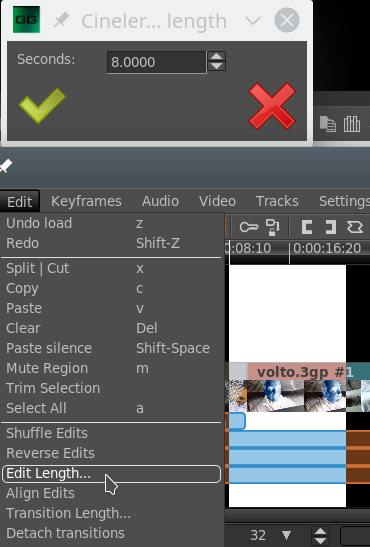
\includegraphics[width=0.6\linewidth]{images/lenght.png}
    \caption{Edit Length window}
    \label{fig:lenght}
\end{figure}

\subsection{Align Edits}%
\label{sub:align_edits}

When loading media, a common problem is that the various audio/video tracks do not always have exactly the same lengths. For example, you might load audio/video recordings from your camera and be dismayed to see that the audio for each segment is a half second longer than the video. If you load a large set of media clips by concatenation, the audio and video will be more skewed as more media is loaded. Align Edits makes it possible to adjust the edits so the audio and/or video align by adjusting 
the edits so that the track lengths are consistent. To use this feature, load all of the desired media and select a region which contains all of the edits to be aligned in the timeline. Now select the menu bar Edit $\rightarrow$ Align Edits menu item to operate the change. The topmost armed track is used as a template reference, and the rest of the tracks are either cut or padded to align the edit boundaries.  Besides aligning audio with the video, you can also align video with the audio if the first armed track is audio. \\
The code performs the following algorithm:
\begin{itemize}
    \item Use the first armed track as the master track (it must contain data).
    \item Collect the \textit{edit project start times} on the selected master track. Only edits that are 100\% inside the selected area will be used.
    \item Set all other tracks to match the \textit{edit times} of the template track, either by putting in silence or cutting the region to align the edits on the \textit{edit times} of the master track.
\end{itemize}
The start time sequence of media and silence edits along the master track are collected as the target 
alignment boundaries. All armed tracks after the master track are modified so that if the next edit edge 
is too soon, it adds silence; if it is too late, edits are shortened or deleted past the point of the next target
alignment boundary time.  Align Edits works best if there are an equal number of Video and Audio sections.  Also, it is better to use cuts instead of adding silence ---if there are silence edits together, the algorithm will combine the silence edits into a single edit and results may not be as desired.

The first two screenshots in figure~\ref{fig:align} show the Before, the Highlighted Edits to be manipulated, and the After results for the Align Edits. The third screenshot \textit{adds silence} in the second section as noted in red letters.
\begin{figure}[htpb]
    \centering
    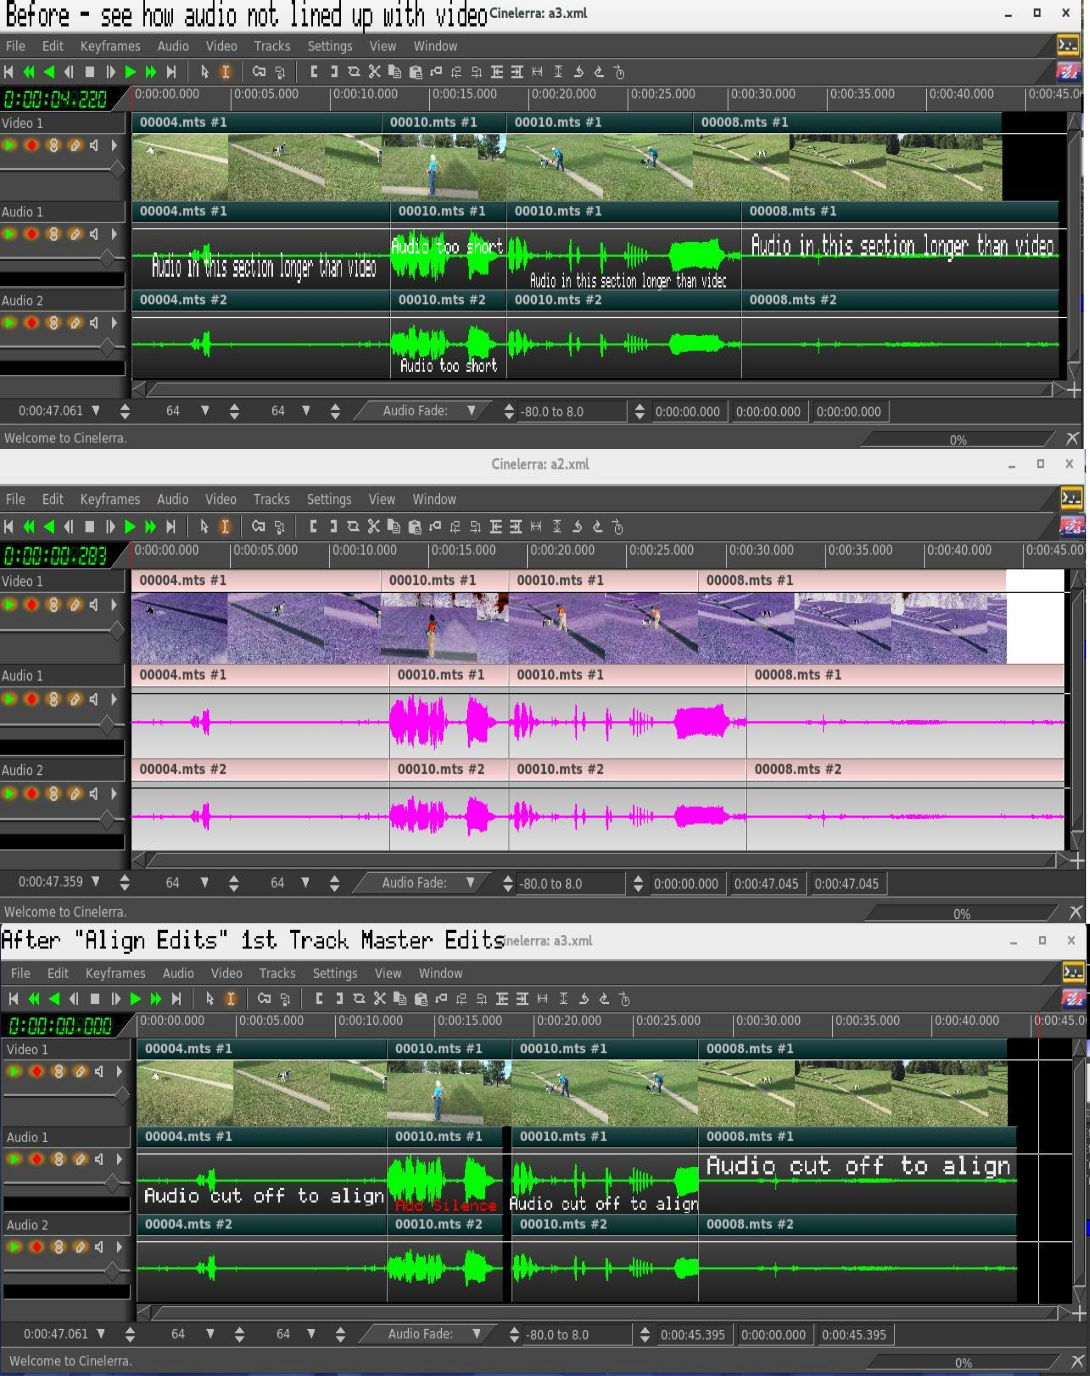
\includegraphics[width=0.8\linewidth]{images/align.png}
    \caption{Align edits}
    \label{fig:align}
\end{figure}

\subsection{Reverse Edits}%
\label{sub:reverse_edits}

The Reverse Edits can be useful to change the order of 2 edits in the case where you would like to put a \textit{teaser} section that occurred in the middle of a movie at the beginning instead, that is, reversed positions.  To operate, highlight completely the edit areas you would like reversed and then use the pulldown Edit $\rightarrow$ Reverse Edits.

Figure~\ref{fig:reverse01} shows the selected / highlighted area to which Edits will be applied.  Note the first edit is 00002, followed by 00003, 00004, and 00005 in that order.
\begin{figure}[htpb]
    \centering
    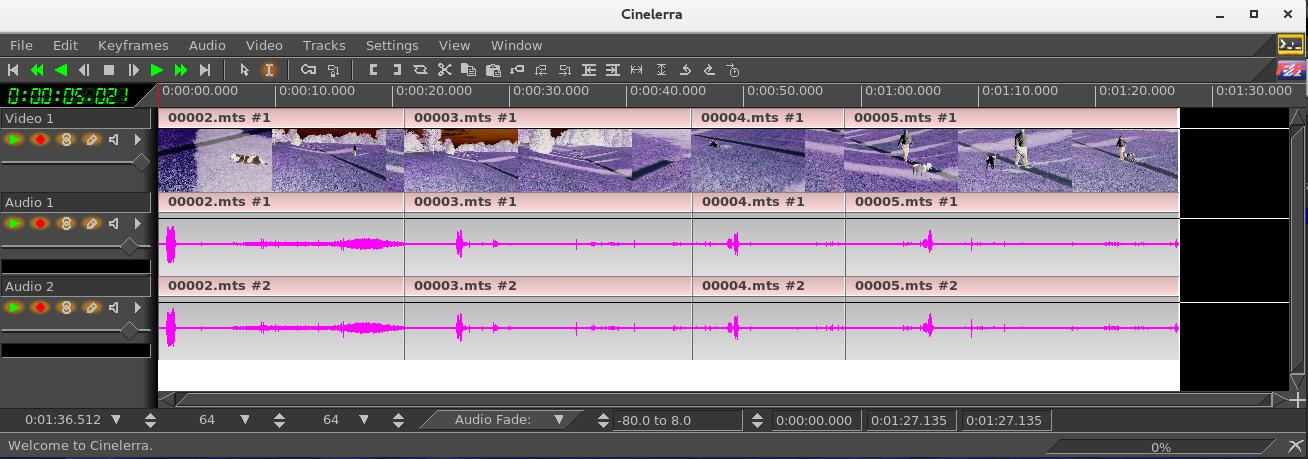
\includegraphics[width=0.8\linewidth]{images/reverse01.png}
    \caption{Selected area for edits aligment}
    \label{fig:reverse01}
\end{figure}

Figure~\ref{fig:reverse02} shows the results of executing \textit{Reverse Edits}.  Now you will see the reversed order of 00005, 00004, 00003, and last 00002.
\begin{figure}[htpb]
    \centering
    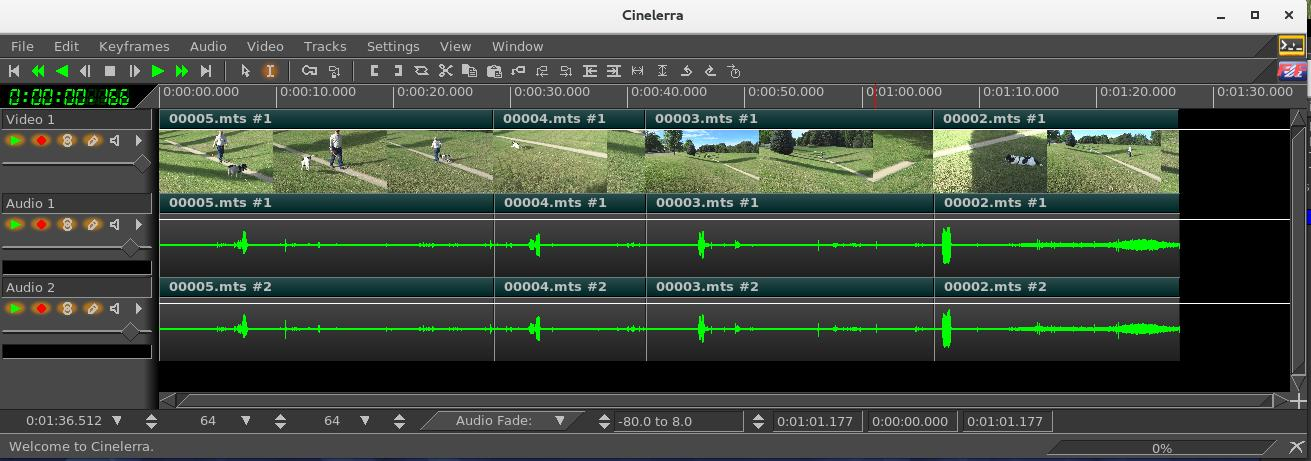
\includegraphics[width=0.8\linewidth]{images/reverse02.png}
    \caption{Results of the Reverse Edits}
    \label{fig:reverse02}
\end{figure}

\subsection{Shuffle Edits}%
\label{sub:shuffle_edits}
 
The file pulldown Edit $\rightarrow$ Shuffle Edits will randomly exchange the location of the edits.  This feature can be used to change the order of the music like you would do from your MP4 player where you have a playlist of your favorite music.  Or perhaps you are creating an advertisement background, you can randomly change it, thus the viewer sees a different order of scenes each time shown.

Figure~\ref{fig:shuffle} illustrating Shuffle Edits of the highlighted area of the first screenshot on the page.  Note the permutation of the fragments resulting in 00003 now being first, then 00005, 00002, and 00004 last.
\begin{figure}[htpb]
    \centering
    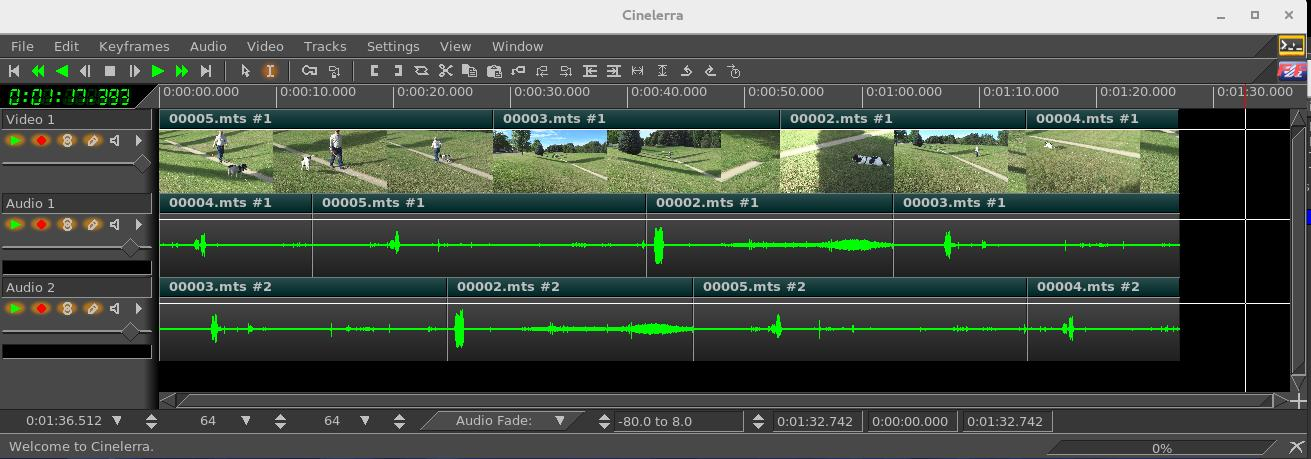
\includegraphics[width=0.8\linewidth]{images/shuffle.png}
    \caption{Shuffle edits: the edits are permutated}
    \label{fig:shuffle}
\end{figure}

\subsection{Drag Handle Management / Trimming}%
\label{sub:drag_handle_management_trimming}

With some edits on the timeline it is possible to do trimming. By trimming you shrink or grow the edit boundaries by dragging them. In drag and drop mode or cut and paste mode, move the cursor over an edit boundary until it changes shape. The drag handle shows as a left or right facing fat arrow when you cursor near the clip start or end.  If the cursor faces left, the dragging operation affects the beginning of the edit. If the cursor faces right, the dragging operation affects the end of the edit.

The effect of each drag operation not only depends on the behavior button but whether the beginning or end of the edit is being dragged. When you release the mouse button, the trimming operation is performed.

For all file formats, other than still images, the extent of the trimming operation is limited to the source file length. Attempting to drag the start of the edit beyond the start of the source, limits it to the source start. In all trimming operations, all edits which start on the same position as the cursor when the drag operation begins are affected. You have to disarm tracks in order to prevent edits from being affected.

You have 6 different choices of which mouse button to use for specific types of editing while using the drag handle.  You change the drag handle mouse effects by using the Settings $\rightarrow$ Preferences  $\rightarrow$ Interface tab and modifying the Editing section as shown in the next figure~\ref{fig:trim}. The drag handle affects not only the clip you are working on but also frequently the entire duration of all clips on the timeline.\\
\begin{figure}[htpb]
    \centering
    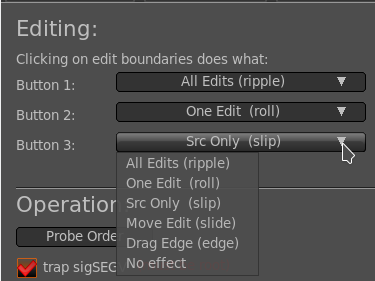
\includegraphics[width=0.6\linewidth]{images/trim.png}
    \caption{Default choices for mouse: Ripple for button 1; Roll for button 2; Slip for button 3}
    \label{fig:trim}
\end{figure}
A description of the fundamental/common terminology for choices follows.
\begin{description}
    \item[All Edits (ripple)] shorten or lengthen the start or end of a single piece of media while moving all media to the right of that clip up or down on the timeline correspondingly.  Timeline duration is modified.  In a drag \textit{All Edits} operation, the beginning of the edit either cuts data from the edit if you move it forward or pastes new data from before the edit if you move it backward. The end of the edit pastes data into the edit if you move it forward or cuts data from the end of the edit if you move it backward. All the following edits shift. If you drag the end of the edit past the start of the edit, the edit is deleted.
    \item[One Edit (roll)] move the in and out point of a single clip without changing the timeline duration. In a drag \textit{One Edit} operation, nothing is cut or pasted. If you move the beginning or end of the edit forward, the source reference in the edit shifts forward. If you move the beginning or end of the edit backward, the source reference shifts backward. The edit remains in the same spot in the timeline but the source shifts.
    \item[Src Only (slip)] move the in and out point of a single clip without changing the timeline duration. In a drag \textit{Src Only} operation, nothing is cut or pasted. If you move the beginning or end of the edit forward, the source reference in the edit shifts forward. If you move the beginning or end of the edit backward, the source reference shifts backward. The edit remains in the same spot in the timeline but the source shifts.
    \item[Slide] a single clip is moved but retains its current in and out point; however the out point of the clip to the left changes and the in point of the clip to the right also changes.  Timeline duration remains the same.
    \item[Edge Left / Right] moves the edge of the clips.
    \item[No effect] no changes are made.  You might want to use this choice to prevent accidental movements.
\end{description}
The next two tables displays the options and results with the Key Table here first.

\vspace{1ex} 
\noindent s = src media start\\
p = proj position \\
l = length \\
c = cut distance \\
rest == p+=c: for rest of clips \\
01 = flags edits\_moved, rest\_moved

\vspace{2ex} \textbf{Cinelerra-HV/CV:}

\begin{figure}[htpb]
    \centering
    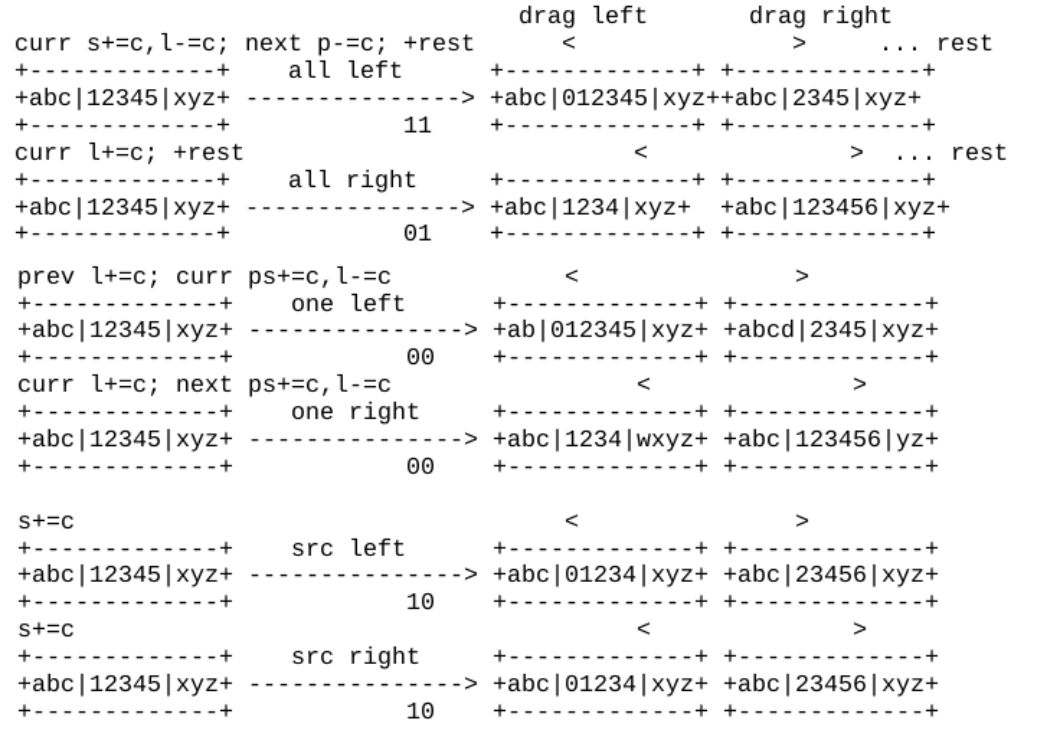
\includegraphics[width=1.0\linewidth]{images/trim-cv.png}
\end{figure}

\vspace{2ex} \textbf{Cinelerra-GG:}

\begin{figure}[htpb]
    \centering
    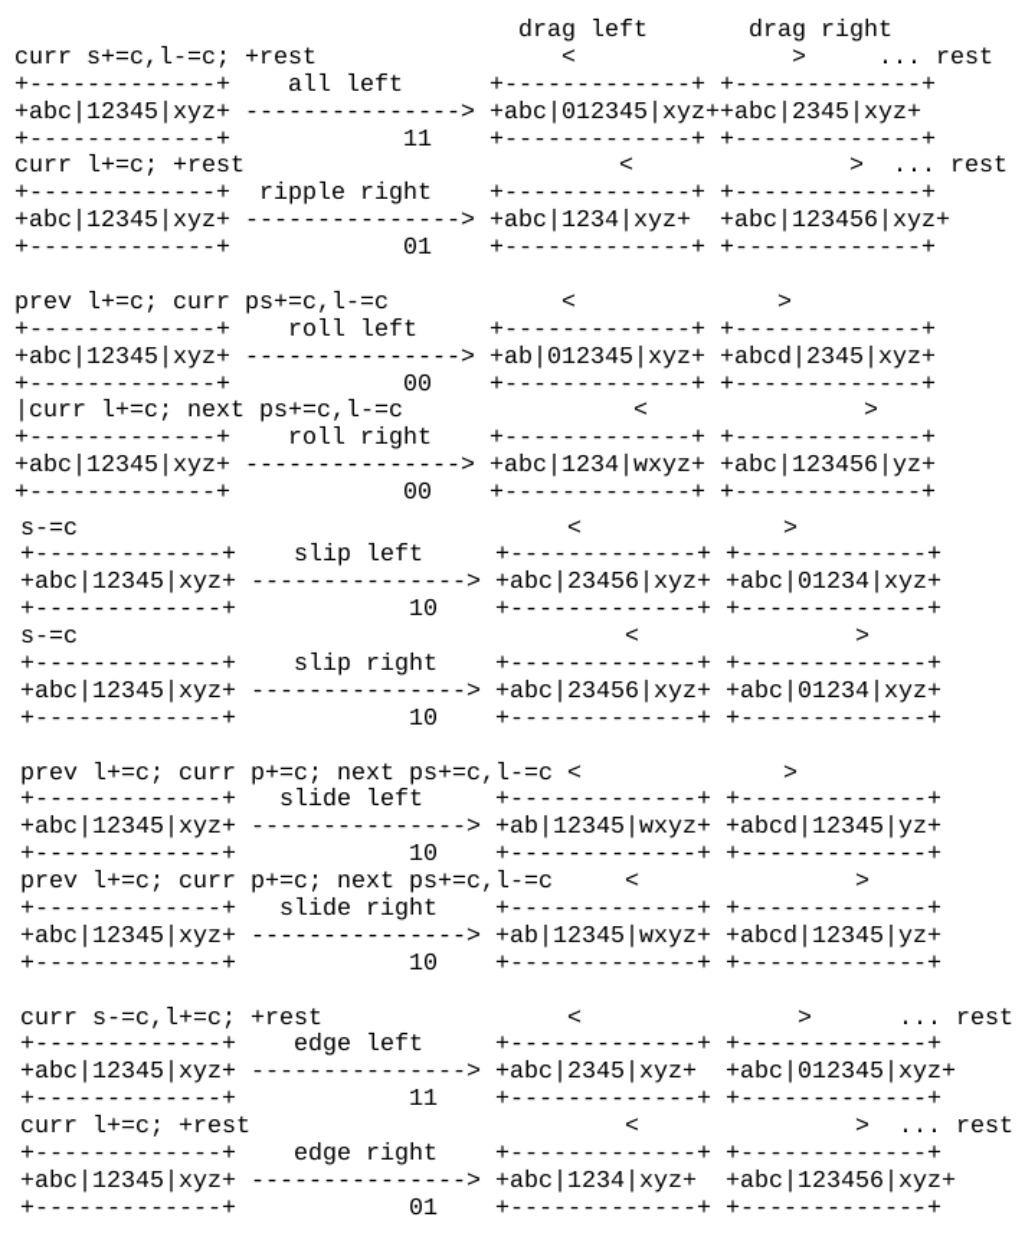
\includegraphics[width=1.0\linewidth]{images/trim-gg.png}
\end{figure}

\paragraph{How to do a J-cut or L-cut} A J-cut is a split edit film editing technique in which the audio from a following scene overlaps the picture from the preceding scene, so that the audio portion of the later scene starts playing before its picture as a lead-in to the visual cut.  An L-cut is a different split edit film editing technique in which the audio from preceding scene overlaps the picture from the following scene, so that the audio cuts after the picture, and continues playing over the beginning of the next scene (figure~\ref{fig:j-cut}). To do either a J-cut or an L-cut, you first shorten the first or second video a little.  Then you block the audio tracks from changing by disarming the appropriate tracks.  Finally use \textit{One Edit (roll)} the cutting edge off the videos.  Moving to the right creates a J-cut and moving to the left creates an L-cut.
\begin{figure}[htpb]
    \centering
    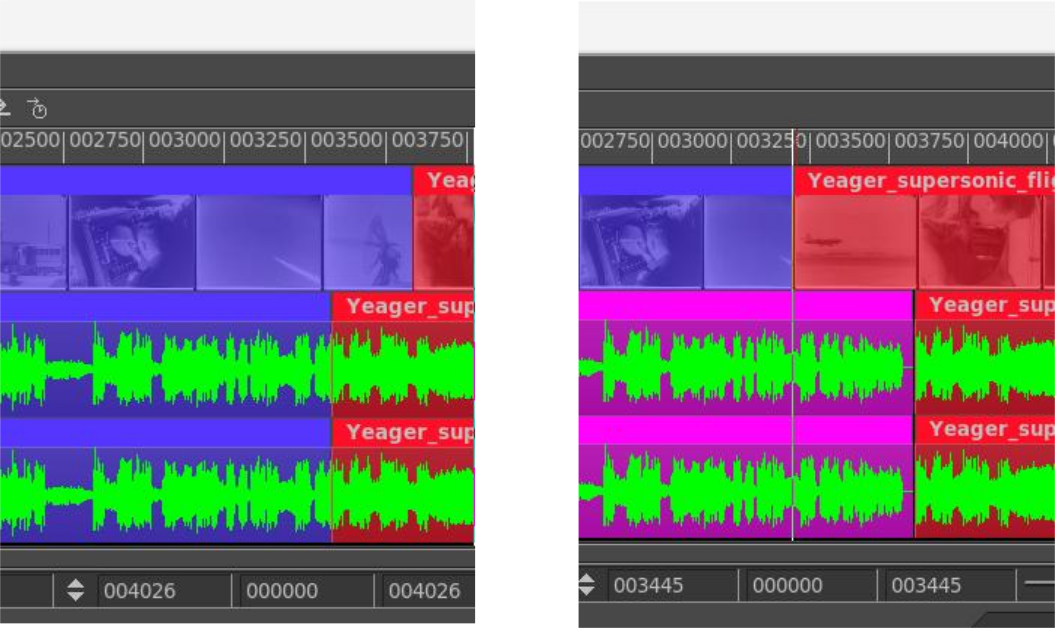
\includegraphics[width=0.8\linewidth]{images/j-cut.png}
    \caption{J-cut to left and L-cut to right}
    \label{fig:j-cut}
\end{figure}

\subsection{Split View in Compositor Using the Drag Handle with Trim}%
\label{sub:split_view_compositor_using_drag_trim}

The Trim Feature using the drag handle provides some good ways to view your video while editing.  The playback position in the compositor is updated live and the view in the compositor can be split so that in the left half of the compositor you can see the last frame of the left clip and in the right half the first frame of the right clip.  Dragging edits can not be extended past the beginning or the end.

First familiarize yourself with button operation; check your setup by executing the following step.  In the Settings $\rightarrow$ Preferences $\rightarrow$ Interface tab, Editing section, clicking on the edit boundaries can be set for Button 1, 2, 3 as one of the following:

\textit{Ripple}; \textit{Roll}; \textit{Slip}; \textit{Slide}; \textit{Edge} or \textit{No effect}

Now to use this feature, create a track with edits that have trims on the left and/or the right. The edit boundary can be modified using \textit{drag handles} at the boundary between the edits (figure~\ref{fig:trim-display}).
\begin{figure}[htpb]
    \centering
    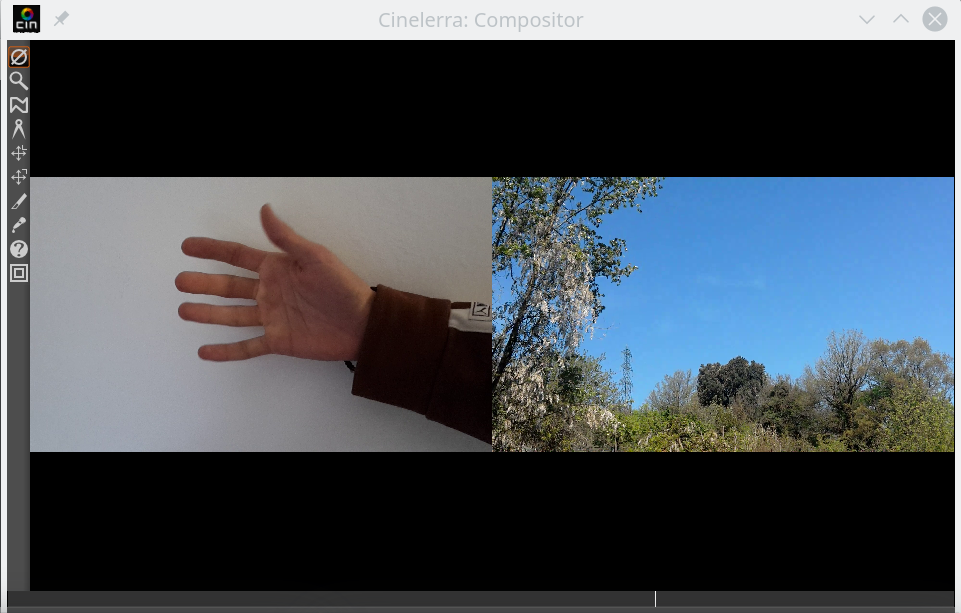
\includegraphics[width=0.9\linewidth]{images/trim-display.png}
    \caption{Split compositor screen showing the result of the Trim feature}
    \label{fig:trim-display}
\end{figure}

\begin{description}
    \item[Left Mouse Button (LMB) usage:] If you grab the edit handle from the right side, you will see a left arrow and dragging the boundary will modify the right edit playback starting time. If you grab the edit handle from the left side, you will see a right arrow and dragging the boundary will modify the left edit playback ending time. In both cases, the composer will show the edit endpoint of the changed edit.
    \item[Shift LMB usage:] The effect on the edits is the same as described above, but the composer will show a split screen of
    the left and right edits as they appear at the drag handle boundary. Dragging will only change one of the two images, since only one edit is being changed.
    \item[Middle Mouse Button (MMB) usage:] Both the left and the right edit ending/starting times are updated.  The image shown in the compositor will be drawn from the side of the drag grab, that is the left if it is grabbed from the left, and the right if it is grabbed from the right.
    \item[Shift MMB usage:] The effect on the edits is the same as described above, but the composer will show a split screen of
    the left and right edits as they appear at the drag handle boundary.  Dragging will change both of the two images, since both edits are being changed.
    \item[Right Mouse Button (RMB) usage:] The start/end point of the current edit is moved, but the edit length is unchanged only one image changes since only one edit endpoint is view is updated.
    \item[Shift RMB usage:] The effect on the edits is the same as described above, but the composer will show a split screen of
    the left and right edits as they appear at the drag handle boundary.  Dragging will only change one of the two images, since only one edit is being changed.
\end{description}

\subsection{Snapping while Cutting and Dragging}%
\label{sub:snapping_cutting_dragging}

\paragraph{Cutting/Snapping edits} cuts from an edit handle to the insert point. 
There are Edit Panel buttons which normally are used to move to the previous or next edit handle/label.
\begin{wrapfigure}[10]{r}{0.5\textwidth}
    \centering
    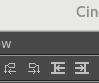
\includegraphics[width=0.6\linewidth]{images/snap.png}
\end{wrapfigure}
They look like tags and the letter E on the menu bar and are oriented forward/backward.  These same buttons can be used to \textit{cut} from the insert pointer to the previous or next edit/label when the \texttt{ctrl+alt} keys are both pressed when the buttons are used.  They \textit{snap} off the media instead of doing the standard re-positioning.  This is useful to minimize the number of operations necessary to cut between edits/labels.

Instead of using the edit panel buttons, you can more easily use the following keyboard shortcuts to perform the same functions:
\begin{center}
    \begin{tabular}{l l l}
        \hline \hline
        snap\_right\_edit &	ctrl+alt+ '.' \\
        snap\_left\_edit &	ctrl+alt+ ',' \\
        snap\_right\_label &	ctrl+alt +shift '.' &  shift+period is the > sign on US keyboards \\
        snap\_left\_label & 	ctrl+alt +shift',' &  shift+comma is the < sign on US keyboards \\
        \hline
    \end{tabular}
\end{center}

\paragraph{Drag Snapping} if you hold down the \texttt{Ctrl + Alt} keys while dragging using the mouse, once the clip gets near to an edit, a label, an in/out pointer or the start/end of the timeline, the dragged clip will snap next to that marker.  The 2 will now be exactly aligned with no gap and no overlap.  As you drag the clip close to one of the markers, when they are within a short distance they start to stick and stay that way until you move further away from that distance.  Also, the line will turn color from green to yellow while in the sticky phase.

\subsection{Nesting}%
\label{sub:nesting}

\paragraph{Nested Assets} A nested asset is an EDL session that embeds an existing EDL session, all tracks, all plugins, editing, and effects into a media object that appears as one audio/video media object, no plugins, editing, or effects.  It is as if the existing EDL was rendered, and loaded in its place.  This has several interesting side effects.  First, you don’t have to render the entire media file to see any portion.  Second, it requires no rendering compute time or storage.  Third, it changes the precedence of the composer so that you get more control over the projection and automation, so that the results can be sent into another rendering step, not simply part of the current stack.  It groups the plugin stack in much the same way that an arithmetic expression is grouped by parenthesis.

The EDL session and the rendered output are visually equivalent.  Nested assets allow for complex grouping and stacking of effects, and makes media access much more flexible.  This feature can be used recursively, that is, any number of sessions may be stacked and referenced as an asset, as long as all of the rendering resources are available.  Nested assets are added to the timeline by using the pulldown File $\rightarrow$ Load files\dots on the main menu and selecting the \textit{Insertion strategy} of \textit{Nest asset}. The file will be pasted into the timeline over the current selection or at the insertion point.

It is somewhat important to note that nested assets and nested clips will have index files automatically created.  These index files can start to clutter up your \texttt{\$HOME/.bcast5} directory with files named \texttt{Nested\_\#\#\#.idx} and you may want to periodically delete any index files which are no longer in use.

\paragraph{Nested Clips} It is also possible to create \textit{clips} and convert them to \textit{nested edl}.  This is done by first creating a clip using the standard cut, clipboard, paste, and/or edit panel buttons.  Now, using the resources \textit{clip} folder, select a clip to be nested, and use the right mouse button to select a clip.  This activates the clip popup menu.  Select the \textit{Nest} menu item, and the clip will be converted to a \textit{Nested: Clip}. Conversely, you can select a \textit{Nested: Clip}, use the \textit{UnNest} menu item, and the clip will be reverted to a \textit{Clip}.  This works similarly to the group / un-group editing features of many graphic design editing programs, but in this case the groups are rendered compositions.  They can not be proxied (figure~\ref{fig:nesting}).
\begin{figure}[htpb]
    \centering
    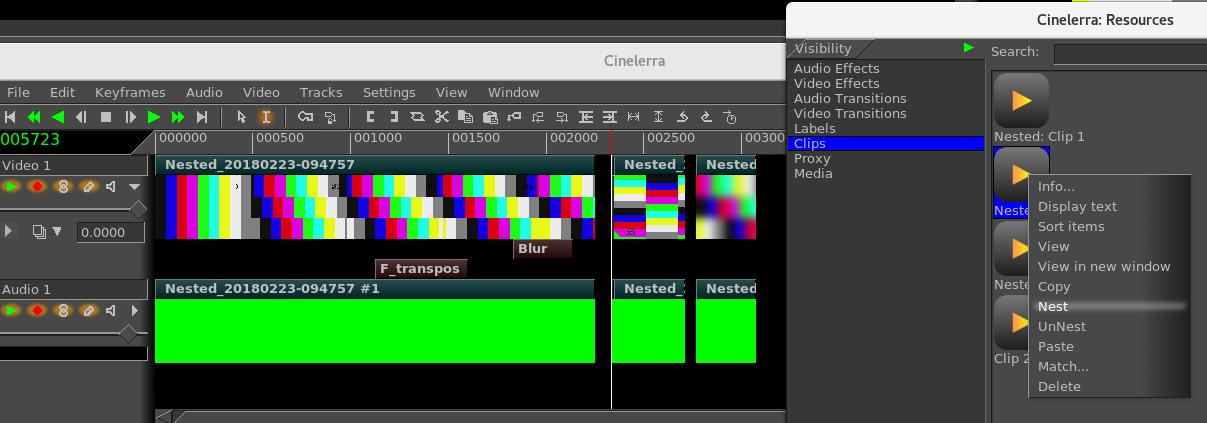
\includegraphics[width=0.9\linewidth]{images/nesting.png}
    \caption{Nested clips in Timeline and Resources window}
    \label{fig:nesting}
\end{figure}

\subsection{Copy/Paste clips/medias across Multiple Instances}%
\label{sub:copy_paste_multiple_instances}

It is easy to copy/paste clips/media within a single instance of cinelerra or across multiple instances.  The reason this works is because there are hidden X cut butters and these are used to transmit EDL from 1 instance to another.

\noindent Steps to copy from a source timeline and paste to a target timeline:

\begin{enumerate}
    \item highlight a selection on the timeline in 1 instance of Cinelerra
    \item use the Copy icon (shortcut c)  on the main menu bar to copy into a buffer
    \item move the pointer to another instance of Cinelerra and set an insertion point in its timeline
    \item use the Paste icon (shortcut v) to paste the clip to that other instance selection target
\end{enumerate}

\section{ShuttlePROv2 and ShuttleXpress Jog Wheels for Editing}%
\label{sec:shuttle_jog_wheels_editing}

\vspace{-2ex} {\footnotesize (credit Eric Messick --- FixedImagePhoto.com/contact)}

\vspace{2ex} The ShuttlePROv2 and ShuttleXpress are affordable jog wheels which can be useful for working with Cin, especially if you do a lot of playing forward/backward, fast/slow/normal, and single frames (figure~\ref{fig:shuttle}).
Directions for using the ShuttlePROv2 and the ShuttleXpress with Cinelerra are described next. These devices work by sending keystrokes used in Cin, corresponding to the shuttle action, to the keyboard buffer. The shuttle has been fully integrated into the Cinelerra code so that after the one initial setup, no further intervention is required.  The multi-speed outer wheel works the same and has the same number of S positions on both shuttles but the shuttle Xpress has only 5 keys.  Since the majority of user operations will most likely be with the use of the 2 wheels, the slightly smaller Xpress could be a better choice with its 5 easy to reach keys.  The Pro is approximately $4x7$\,inches whereas the Xpress is about $4x4$\,inches.
\begin{figure}[htpb]
    \centering
    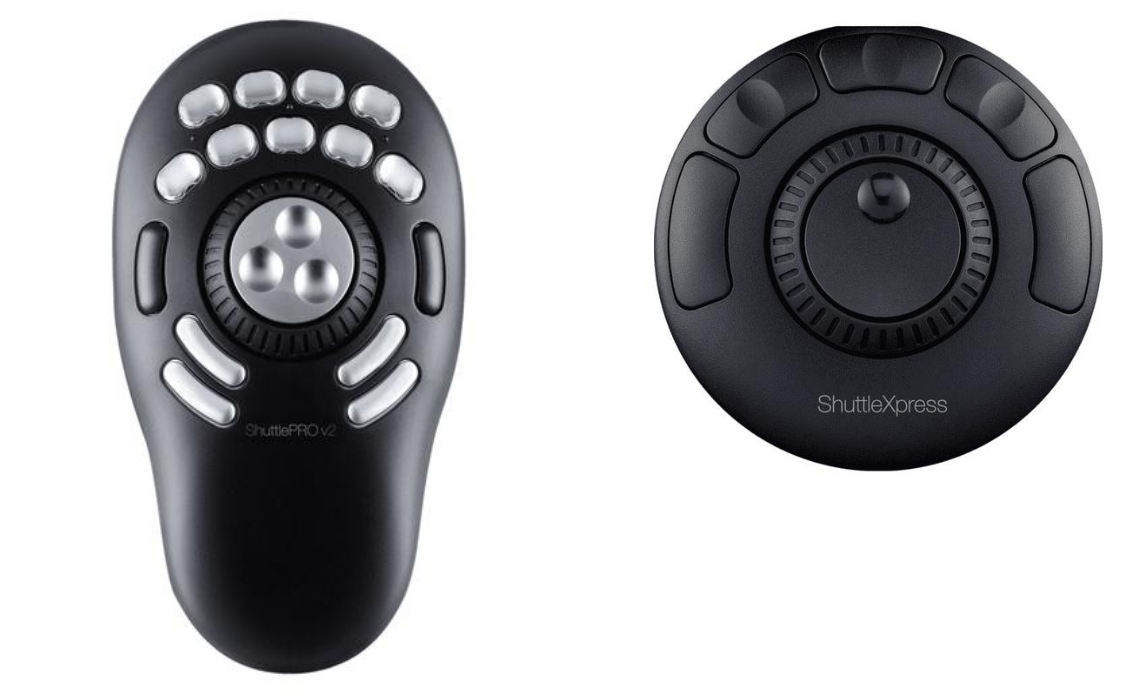
\includegraphics[width=0.9\linewidth]{images/shuttle.png}
    \caption{ShuttlePROv2 and ShuttleXpress}
    \label{fig:shuttle}
\end{figure}

\noindent The vendor supplied \textit{string} device names for the shuttles are currently:

\vspace{1ex} \texttt{/dev/input/by-id/usb-Contour\_Design\_ShuttlePRO\_v2-event-if00}
 
 \texttt{/dev/input/by-id/usb-Contour\_Design\_ShuttleXpress-event-if00}
 
 \texttt{/dev/input/by-id/usb-Contour\_Design\_ShuttlePro-event-if00}

\vspace{1ex}
\noindent Only 1 necessary initial setup is required due to permission settings for non-root usage. As root, just copy a file that provides the necessary permissions to use the shuttle, then reboot,  Example copy:

\begin{lstlisting}[language=Bash]
  sudo cp {cindat_path}/doc/99-ShuttlePRO.rules   /etc/udev/rules.d/
\end{lstlisting}

\noindent then the next time after you reboot, the permissions should be correct. This file only needs to contain one of the following lines depending on which shuttle version you have/use, but all will be in the file.

\begin{lstlisting}[language=Bash]
ATTRS{name}=="Contour Design ShuttlePro" MODE="0644"		# for  newer PRO model \\
ATTRS{name}=="Contour Design ShuttlePRO v2" MODE="0644"	# for older PRO model \\
ATTRS{name}=="Contour Design ShuttleXpress" MODE="0644"	# for the Xpress model \\
SUBSYSTEMS=="usb", ATTRS{idVendor}=="0b33", ATTRS{idProduct}=="0020", MODE="0666" \\
SUBSYSTEMS=="usb", ATTRS{idVendor}=="0b33", ATTRS{idProduct}=="0030", MODE="0666"
\end{lstlisting}

\noindent If you swap your shuttle, for example upgrade from an Xpress to a PROv2, just stop Cin, unplug the original shuttle, plug in the replacement shuttle, and restart Cin.  If you start the cinelerra program and the shuttle does not function as before, stop cinelerra and then simply unplug it and plug it in again.  There are a couple of reasons why it may stop functioning.  One is because cinelerra was not stopped with the usual Quit command and the shuttle was improperly shut down when there was a crash.  The other possibility is that a static discharge occurred in the area.

A default shuttlerc file is automatically used when a shuttle device is plugged in when Cin is started. This file sets up the key bindings for Cinelerra to use. You can override any default settings by having a local file in your \texttt{\$HOME} directory, named \texttt{.shuttlerc} to reflect your personal preferences.

\subsection{How to Modify the Default Key Settings}%
\label{sub:modify_default_key_settings}

Detailed information on how to modify your local .shuttlerc file is described next, but if you need help you can request more information in the forum at \url{https://cinelerra-gg.org}. In the \texttt{shuttlerc} file, a \# always represents a comment and blank lines are ignored.  The first thing you must do is copy the system supplied \texttt{shuttlerc} file to your \texttt{\$HOME} directory and rename it as \texttt{.shuttlerc} (with a period). 

The \texttt{shuttlerc} file has sections that in the case of Cinelerra, represent different windows allowing you to set the keys, K1-K15 for the Pro and K5-K9 for the Xpress, the shuttle wheel positions of S0/S1/S-1 for stop, S2 through S7 for wheeling to the right, and S-7 through S-2 for wheeling to the left for reverse.  Then there is JR to jog right (clockwise) and JL to jog left (counter-clockwise) for the inner smaller wheel for single frame movement.  See the key arrangement on a later page for location of the keys for each of the two different shuttles.

The sections are surrounded by brackets for windows such as Cinelerra (the main window), Viewer, Composer, Resources, Load, and Default.  If you want the keys to be defined the same in every window, you can bracket each window on lines one right after the other and then just define one set of keys.  The other lines will have the key name/shuttle position followed by its assigned value.  The values you use for the keys are usually shortcuts and have to be operationally defined within Cinelerra. For example, the shortcut “f” to go fullscreen is defined so can be used; however the shortcut “h” is not defined so will not do anything.  You can check the file, shortcuts.html, for some options to use.

Next are a few actual examples from the default \texttt{{cindat\_path}/shuttlerc} file.

\noindent The next brackets represent sections. Default, Resources, Load windows all use the same key values.

\begin{lstlisting}[language=Bash]
[Default] \\
[Resources] \\
[Load] \\
K5 XK_Home \\
K6 XK_Button_1	# same as mouse button 1 \\
K7 XK_Button_2	# same operation as mouse button 2 \\
K8 XK_Button_3 \\
K9 XK_End \\
JL XK_Scroll_Up	# for example, in the Load menu, use scroll up to get to the next file name \\
JR XK_Scroll_Down
\end{lstlisting}

\noindent Cinlerra with brackets around it next, is the section with some key definitions for the main window.

\begin{lstlisting}[language=Bash]
[Cinelerra] \\

# Most useful functions have to be on K5-K9 because Xpress only has 5 keys \\
K5 XK_Home  	# Beginning \\
K6 XK_KP_6 	# Reverse, or if playing Stop \\
K7 XK_KP_0  	# Stop \\
K8 XK_KP_3   	# Play, or if playing Stop \\
K9 XK_End       	# End \\
... \\
S-7 REV_16     	# Next 6 are reverse keys \\
S-6 REV_8      	#  the number on the end represents speed\\
S-5 REV_4      	#  number can be decimal up to 64 \\
S-4 REV_2      	#  2 means 2x or double speed \\
S-3 REV_1 \\
S-2 REV_0.5    	#  0.5 represents 1/2 speed \\
S-1 XK_KP_0    	# Because the Shuttle does not generate S0, have to use S-1 \\
S0  XK_KP_0   	# Hardware does not generate S0 \\
S1  XK_KP_0   	# Because the Shuttle does not generate S0, have to use S1 \\
S2  FWD_0.5 \\
S3  FWD_1 \\
... \\
\end{lstlisting}

\noindent An explanation for the above REV and FWD key symbol values is necessary to facilitate user preferences.  Obviously REV stands for reverse and FWD for forward.  You can set any speed up to and including 64x (that is, 64 times the normal speed) on any of the S keys.  First in the line is the key name such as S-3 and then the key direction of FWD or REV followed by the symbol for underscore (\_) and then the numerical value to use.  For example, if you want the 5\textsuperscript{th} forward position, S5, to play 10$ \frac{1}{2}$ times faster, you would use the statement \texttt{S5 FWD\_10.5}.  Integer or decimal numbers are legal.

For the Viewer, you may want keys defined to do a Splice or an Overwrite so define differently.  Note that assignments that contain single character letters must be enclosed in quotes.

\begin{lstlisting}[language=Bash]
[Viewer] \\
K2 "v"         # Splice - Viewer only; may be defined differently than Composer or Cinelerra \\
K4 "b"         # Overwrite
\end{lstlisting}

\noindent To change any key value to an alternative value, just edit the file and make the changes.  Besides just keys and alphabetic letters of numbers, you can also use any cinelerra value that contains the combination with Shift, Alt, and Ctrl.  For keys that are not printable characters, you can look up the symbol name to use for a specific operation in the file called: \texttt{/usr/include/X11/keysymdef.h} .
\noindent Some examples:

\begin{lstlisting}[language=Bash]
K10 Alt-XK_Left  	# Go to previous edit \\
K13 Ctrl-XK_Right 	# Go to next label
\end{lstlisting}

\noindent For sequences of one or more \textit{printable} characters, you can just enclose them in double quotes.  For example in the \texttt{[Composer]} section, to go into or out of fullscreen mode, automatically start playing and put a label there, you could define a key like this:  K7 “f l” - that is printable character f, a space, and printable character l.  

After modifying \texttt{.shuttlerc}, the next time you use the shuttle, your changes will automatically take affect without even having to stop and restart Cin.  However, the first thing to try if problems is to stop cinelerra, unplug the shuttle, wait a few seconds, plug it in again, and then restart cin.  If for some reason, the shuttle keys still do not work after that, you may have an incorrect setup and you will have to correct that first.  For example, if you define S5 twice within the Cinelerra setup, it will fail.  It is suggested that if you make changes, you should initially uncomment DEBUG in the \texttt{.shuttlerc} file and start up cinelerra from a terminal window so that you can make sure it is working and has no output errors.  An error might look like:

\begin{lstlisting}[language=Bash]
dupl key name: [Cinelerra]K1 \\
shuttle config err file: /root/.shuttlerc, line:37
\end{lstlisting}

\noindent Keep in mind when changing the values, that the ShuttleXpress has fewer buttons so if you define K1 it will only work for the ShuttlePro. 

Any time you are having trouble with your shuttle, you can copy the default \texttt{shuttlerc} file from \texttt{{cindat\_path}/shuttlerc} to your local \texttt{.shuttlerc} file, and edit that to\ switch to DEBUG mode by removing the \# comment from the DEBUG line.  But you will have to have started Cin from a terminal window to see the key values. The first time you use the shuttle or after you change the file, the current assignments will show in the terminal window so will look something like:

\begin{lstlisting}[language=Bash]
[Cinelerra] # 1 \\
K5[D]: XK_KP_0/U \\
K5[U]: XK_KP_0/U 
\end{lstlisting}

\noindent When you are in DEBUG mode and are just working away, what you will see is something like this:

\begin{lstlisting}[language=Bash]
key: 0058 1 \\
key: 0055 0
\end{lstlisting}

or:

\begin{lstlisting}[language=Bash]
shuttle:  00 00 00 00 00 \\
key: XK_Home 0
\end{lstlisting}

\noindent When you change the focus from one window to another, you will see something like this:

\begin{lstlisting}[language=Bash]
new focus: 04c00137 \\
new translation: Viewer \\
key: 0059 1
\end{lstlisting}

\noindent You can also set an environment variable to temporarily use an alternative shuttle configuration file for testing as in:

\begin{lstlisting}[language=Bash]
export SHUTTLE_CONFIG_FILE=/tmp/shuttlerc_test 
\end{lstlisting}

\noindent The shuttle wheel occasionally will not \textit{stop} after you have wheeled it to play forward.  This is a documented known problem from the original code so you just have to joggle it a little in the other direction and then it will stop.  S0 does not always generate a signal to do a stop and that is why S1 and S-1 have to be used to relay the stop instead.  Also, if you have a fullscreen Composer or Viewer up and the regular one also, the fullscreen takes precedence.

\subsection{Troubleshooting auxilliary information}%
\label{sub:troubleshooting_auxilliary_information}

In order to see if you hardware was recognized by the operating system, keyin:

\begin{lstlisting}[language=Bash]
lsusb -v -d 0b33:0030		# for the Shuttle Pro or PROv2 \\
lsusb -v -d 0b33:0020		# for the Shuttle Xpress
\end{lstlisting}


\paragraph{Note 1} Currently, the keys K14 and K15 do not function on the \textit{Contour Design ShuttlePro} but do on the   \textit{Contour Design ShuttlePRO v2} due to a Report Descriptor error.  You can workaround this by uncommenting \texttt{USB\_DIRECT} in your local \texttt{.shuttlerc} file.  This directly uses libusb rather than the generic Linux hid driver.  \texttt{USB\_DIRECT} works for any of the currently tested shuttles. 
    
\paragraph{Note 2} If you are not sure if your shuttle is fully functional, you can verify that the hardware device has been seen by your operating system with this procedure.


\begin{enumerate}
    \item From a terminal window as an ordinary user keyin:  lsusb  (the first character is a lower case L ---for
    list).  You will see something like the following depending on which usb device you have the
    ShuttlePro plugged into:
    
    \texttt{Bus 003 Device 002: ID 0b33:0030 Contour Design, Inc. ShuttlePro v2}
    \item To make sure you have usbmon installed keyin:
    
    \texttt{sudo modprobe usbmon}
    \item Next keyin the following:
    
    \texttt{sudo od -tx1 /dev/usbmon3} 
    
    where the last 3 is the same \# as the Bus in above.  If it lists \texttt{Bus 002}, then use \texttt{/dev/usbmon2} instead.
    \item Now with focus in that same terminal window, press any shuttle key just to see what happens and
    should see about 12 lines similar to these below ---a new set every time you press a single key or the
    wheel.  The lines are usually not important, just the fact that you get a response is.  However if you
    have multiple devices on the same bus, you will get responses from any and all of them.  Attempt to
    isolate your shuttle by temporarily unplugging unnecessary devices on the same bus or plug the 
    shuttle into a different usb port that has fewer devices.
    \begin{lstlisting}[language=Bash]
       0000000 80 70 99 75 53 8c ff ff 43 01 81 02 03 00 2d 00 \\
       0000020 4e 61 5c 5c 00 00 00 00 8d 2c 06 00 00 00 00 00 \\
       0000040 05 00 00 00 05 00 00 00 00 00 00 00 00 00 00 00 \\
       0000060 01 ff 00 00 00 80 70 99 75 53 8c ff ff 53 01 81 \\
       0000100 02 03 00 2d 3c 4e 61 5c 5c 00 00 00 00 b1 2c 06 \\
       0000120 00 8d ff ff ff 05 00 00 00 00 00 00 00 00 00 00 \\
       0000140 00 00 00 00 00 80 70 99 75 53 8c ff ff 43 01 81 \\
       0000160 02 03 00 2d 00 4e 61 5c 5c 00 00 00 00 3d d7 09 \\
       0000200 00 00 00 00 00 05 00 00 00 05 00 00 00 00 00 00 \\
       0000220 00 00 00 00 00 00 ff 00 00 00 80 70 99 75 53 8c \\
       0000240 ff ff 53 01 81 02 03 00 2d 3c 4e 61 5c 5c 00 00 \\
       0000260 00 00 64 d7 09 00 8d ff ff ff 05 00 00 00 00 00
    \end{lstlisting}
    \item Next press the key that you want to verify is functioning --- if no new lines show up, then the key is
    non-functional so there is a hardware problem.  If you get output, then perhaps there is a problem
    with your software setup.
    \item Use Ctrl-C on the terminal window when done to get back to the prompt.
\end{enumerate}
\paragraph{Note 3}
Another method for testing to make sure your model of the Shuttle does not have different key definitions than the one that Cinelerra was coded for is to do the following.

\begin{enumerate}
    \item Locate the shudmp.C program in your Cinelerra directory.
    \item Compile that with the command:  \texttt{c++ shdmp.C -o shudmp}
    \item Make the file executable with the command:  \texttt{chmod +x shudmp}
    \item \texttt{sudo ./shdmp /dev/input/by-id/usb-Contour\_Design\_ShuttlePro-event-if00   \# substitute your shuttle}
\end{enumerate}

\noindent Then press your shuttle key that is having problems and check the results.  They should look like:

\begin{lstlisting}[language=Bash]
Example for K7: \\
event: (4, 4, 0x90007)		#The last number, 7, is the expected Key number. \\
event: (1, 262, 0x1) \\
event: (0, 0, 0x0) \\
event: (4, 4, 0x90007) \\
event: (1, 262, 0x0) \\
event: (0, 0, 0x0) \\

Example for K15: \\
event: (4, 4, 0x9000f)		#The last number f is 15 in octal and is the expected Key. \\
event: (1, 270, 0x1) \\
event: (0, 0, 0x0) \\
event: (4, 4, 0x9000f) \\
event: (1, 270, 0x0) \\
event: (0, 0, 0x0)
\end{lstlisting}

\noindent When done, you will have to Ctrl-C to get out of the program.

\paragraph{Note 4} For developers, it is also possible to do the following for further in depth testing:

\begin{enumerate}
    \item \texttt{ls /sys/kernel/debug/hid   \# to locate numerical value of the shuttle, e.g. 0003:0B33.0030.0006}
    \item \texttt{cat “/sys/kernel/debug/hid/0003:0B33.0030.0006/rdesc”    \# substitute your own numerical value}
    \item \texttt{cat “/sys/kernel/debug/hid/0003:0B33.0030.0006/events”  \# press keys to see the results}
\end{enumerate}

\subsection{Shuttle key default arrangement for Cinelerra / Composer / Viewer:}%
\label{sub:shuttle_key_default_cinelerra}

The following is the default setting for the ShuttlePROv2 and ShuttleXpress:

\vspace{1ex} \textbf{ShuttlePROv2:}

\begin{figure}[t]
    \centering
    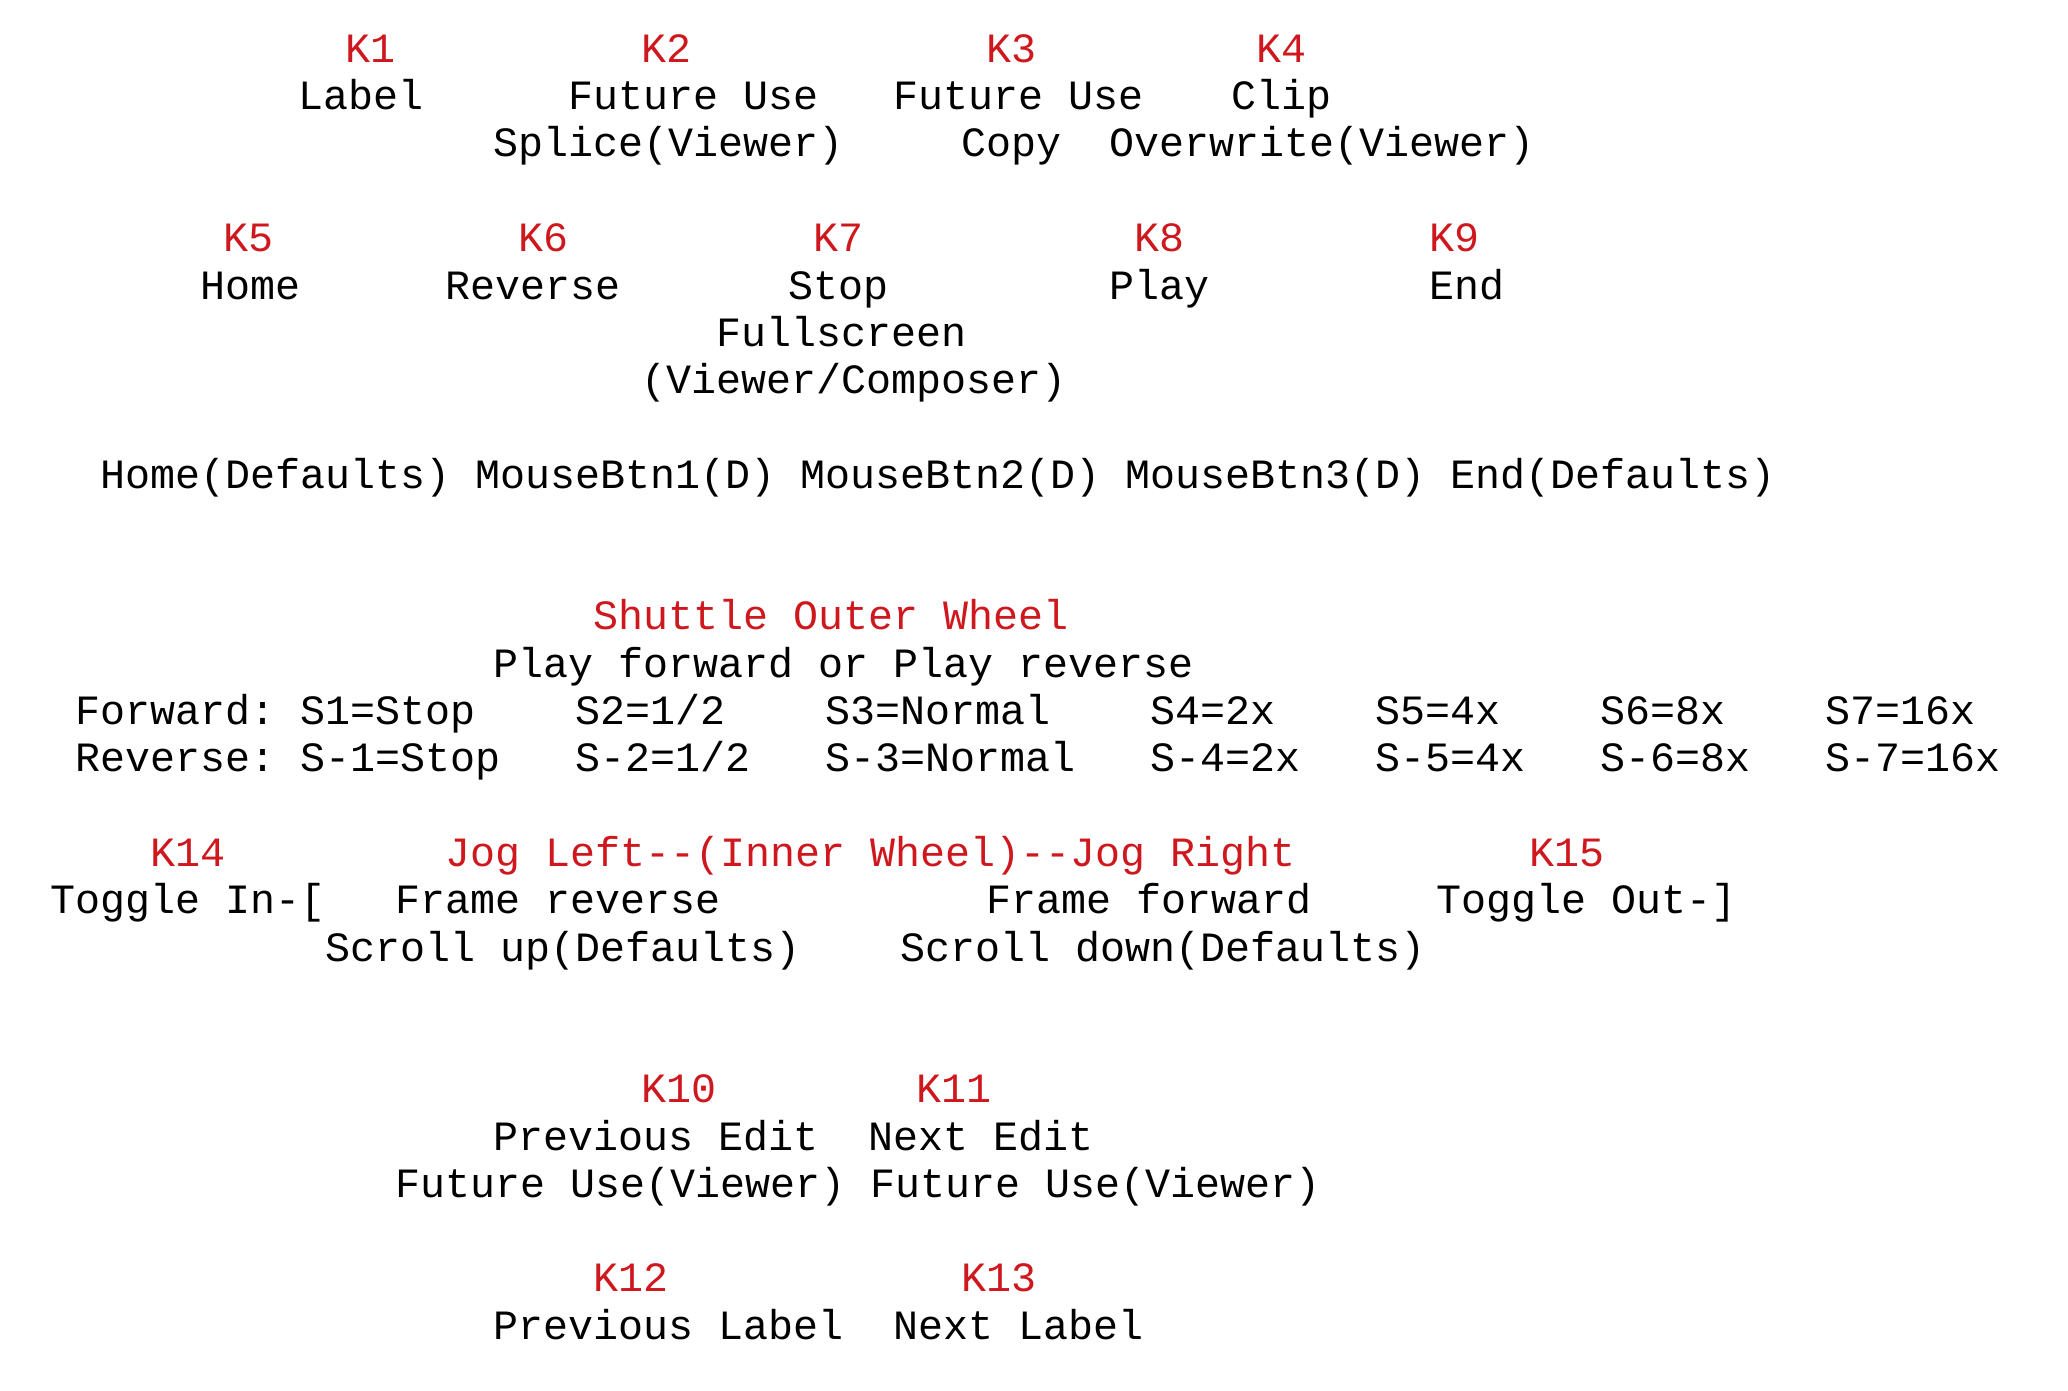
\includegraphics[width=1.0\linewidth]{images/shuttle-prov2.png}
\end{figure}

\vspace{1ex} \textbf{ShuttleXpress:}

\begin{figure}[b]
    \centering
    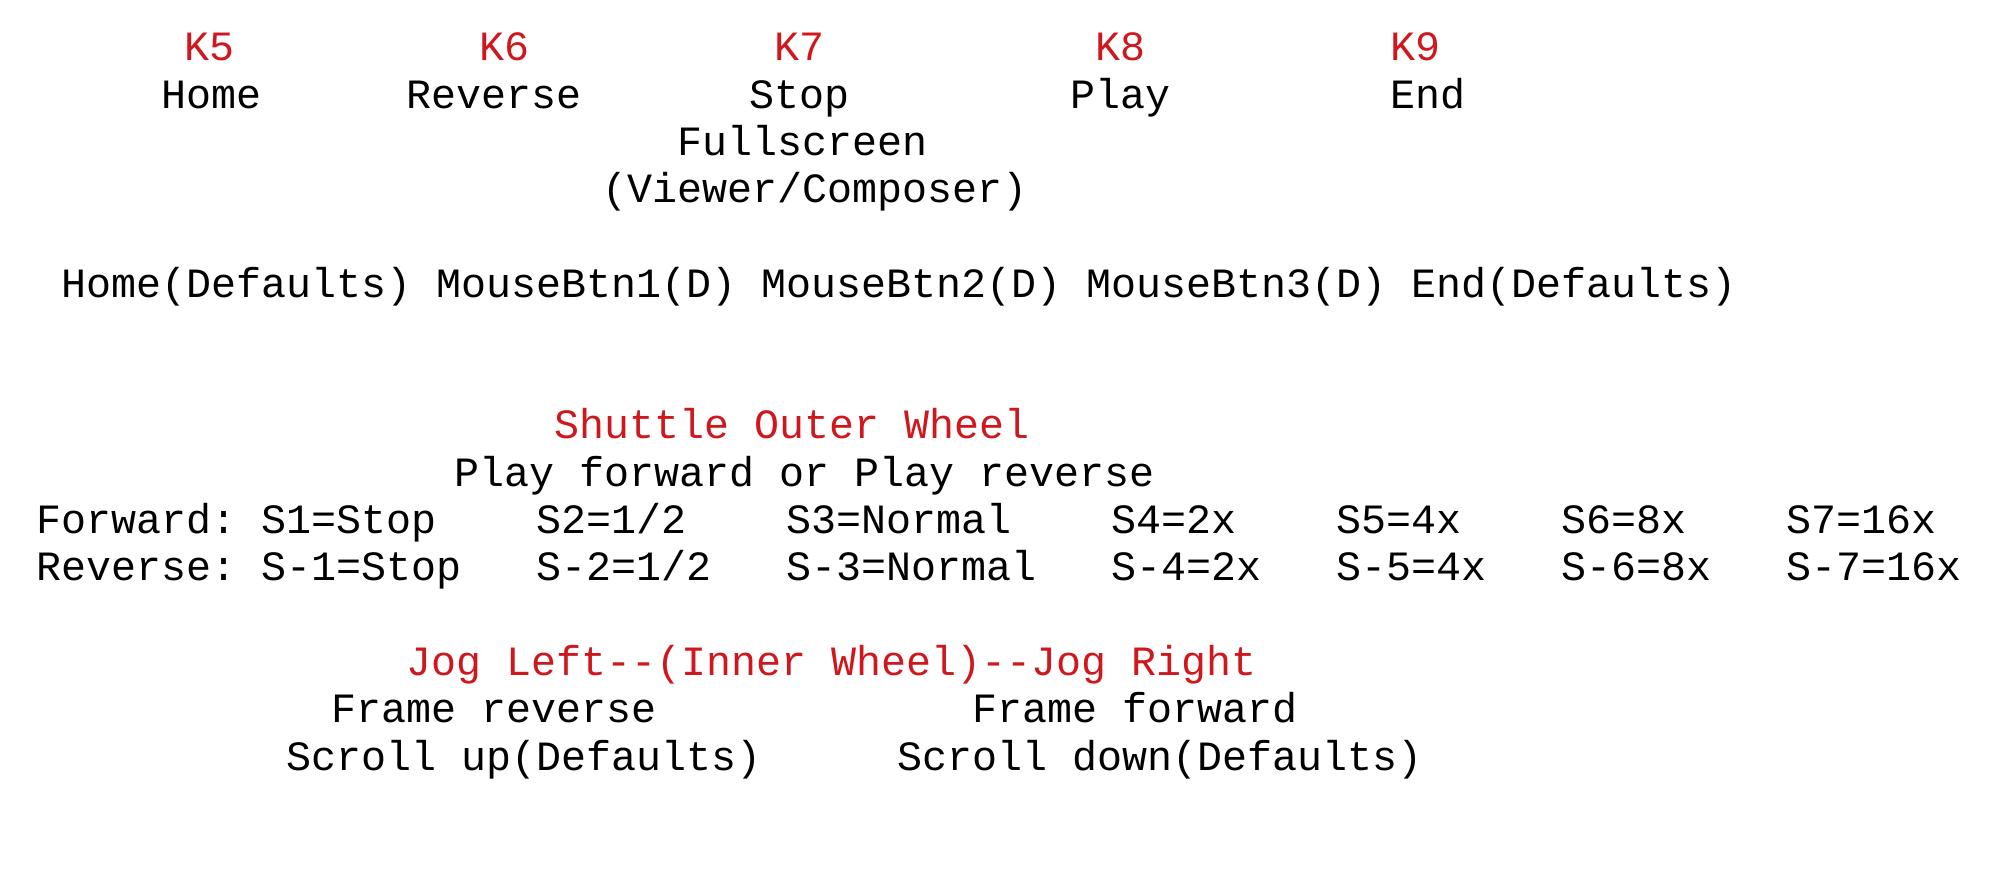
\includegraphics[width=1.0\linewidth]{images/xpress.png}
\end{figure}
